\section{华为云实验环境}

课程设计实验主要用到华为云的 SWR、CCE、OBS 和 ELB。SWR 保存后端和前端镜像，CCE 提供 Kubernetes 集群，OBS 作为 Spark 数据读取的一种来源，ELB 用来给后端服务提供公网入口。后续部署能否跑通，基本都取决于这些资源是否先配置正确，例如 Kubernetes 版本、Worker 节点数量、节点 Ready 状态和公网访问入口。

实验区域选择华北-北京四，创建的 CCE Standard 集群名称为 \texttt{cloud-course-cce}。集群同时配置了 VPC、子网、两个 Worker 节点和负载均衡资源。为了控制代金券消耗，Worker 节点采用 2 vCPU / 4 GiB 规格；Kubernetes 版本和节点数量仍满足任务书要求。集群创建完成后，我们在 CloudShell 中检查了节点列表、集群连接信息和 kubectl 客户端版本，确认后再继续部署应用。

\subsection{云服务与资源配置}

表 \ref{tab:cloud-env-summary} 列出了本次实验实际用到的几类云服务。

\begin{table}[H]
  \centering
  \caption{华为云实验环境资源概览}
  \label{tab:cloud-env-summary}
  \small
  \renewcommand{\arraystretch}{1.22}
  \begin{tabularx}{\textwidth}{>{\raggedright\arraybackslash}p{2.0cm} >{\raggedright\arraybackslash}p{2.6cm} Y}
    \toprule
    云服务 & 本项目用途 & 关键配置或说明 \\
    \midrule
    SWR & 容器镜像仓库 & 保存 \texttt{backend:v1} 与 \texttt{frontend:v1} 镜像，为 CCE Deployment 提供镜像来源。 \\
    CCE & Kubernetes 集群 & 创建 \texttt{cloud-course-cce} 集群，版本为 v1.34，包含 2 个 Worker 节点。 \\
    OBS & Spark 数据存储接口 & Spark 脚本支持通过 \texttt{s3a://} 路径读取数据；当前报告中 Spark 章节将结合数据分析脚本展开说明。 \\
    ELB & 公网负载均衡 & 后端 \texttt{backend-svc} 通过共享型公网 ELB 暴露 \texttt{/api/ping} 接口。 \\
    \bottomrule
  \end{tabularx}
\end{table}

\subsubsection{SWR镜像仓库配置}

SWR 是本项目中连接本地容器构建与云端 Kubernetes 部署的关键环节。后端 Flask 服务和前端 Nginx 服务在本地完成 Docker 镜像构建后，需要推送至华为云 SWR，随后 CCE 节点才能在创建 Pod 时从私有镜像仓库拉取镜像。由于 SWR 镜像仓库通常为私有仓库，后续 Deployment 中还需要结合镜像拉取密钥或 CCE 自动生成的 \texttt{default-secret} 进行鉴权。

\begin{figure}[H]
  \centering
  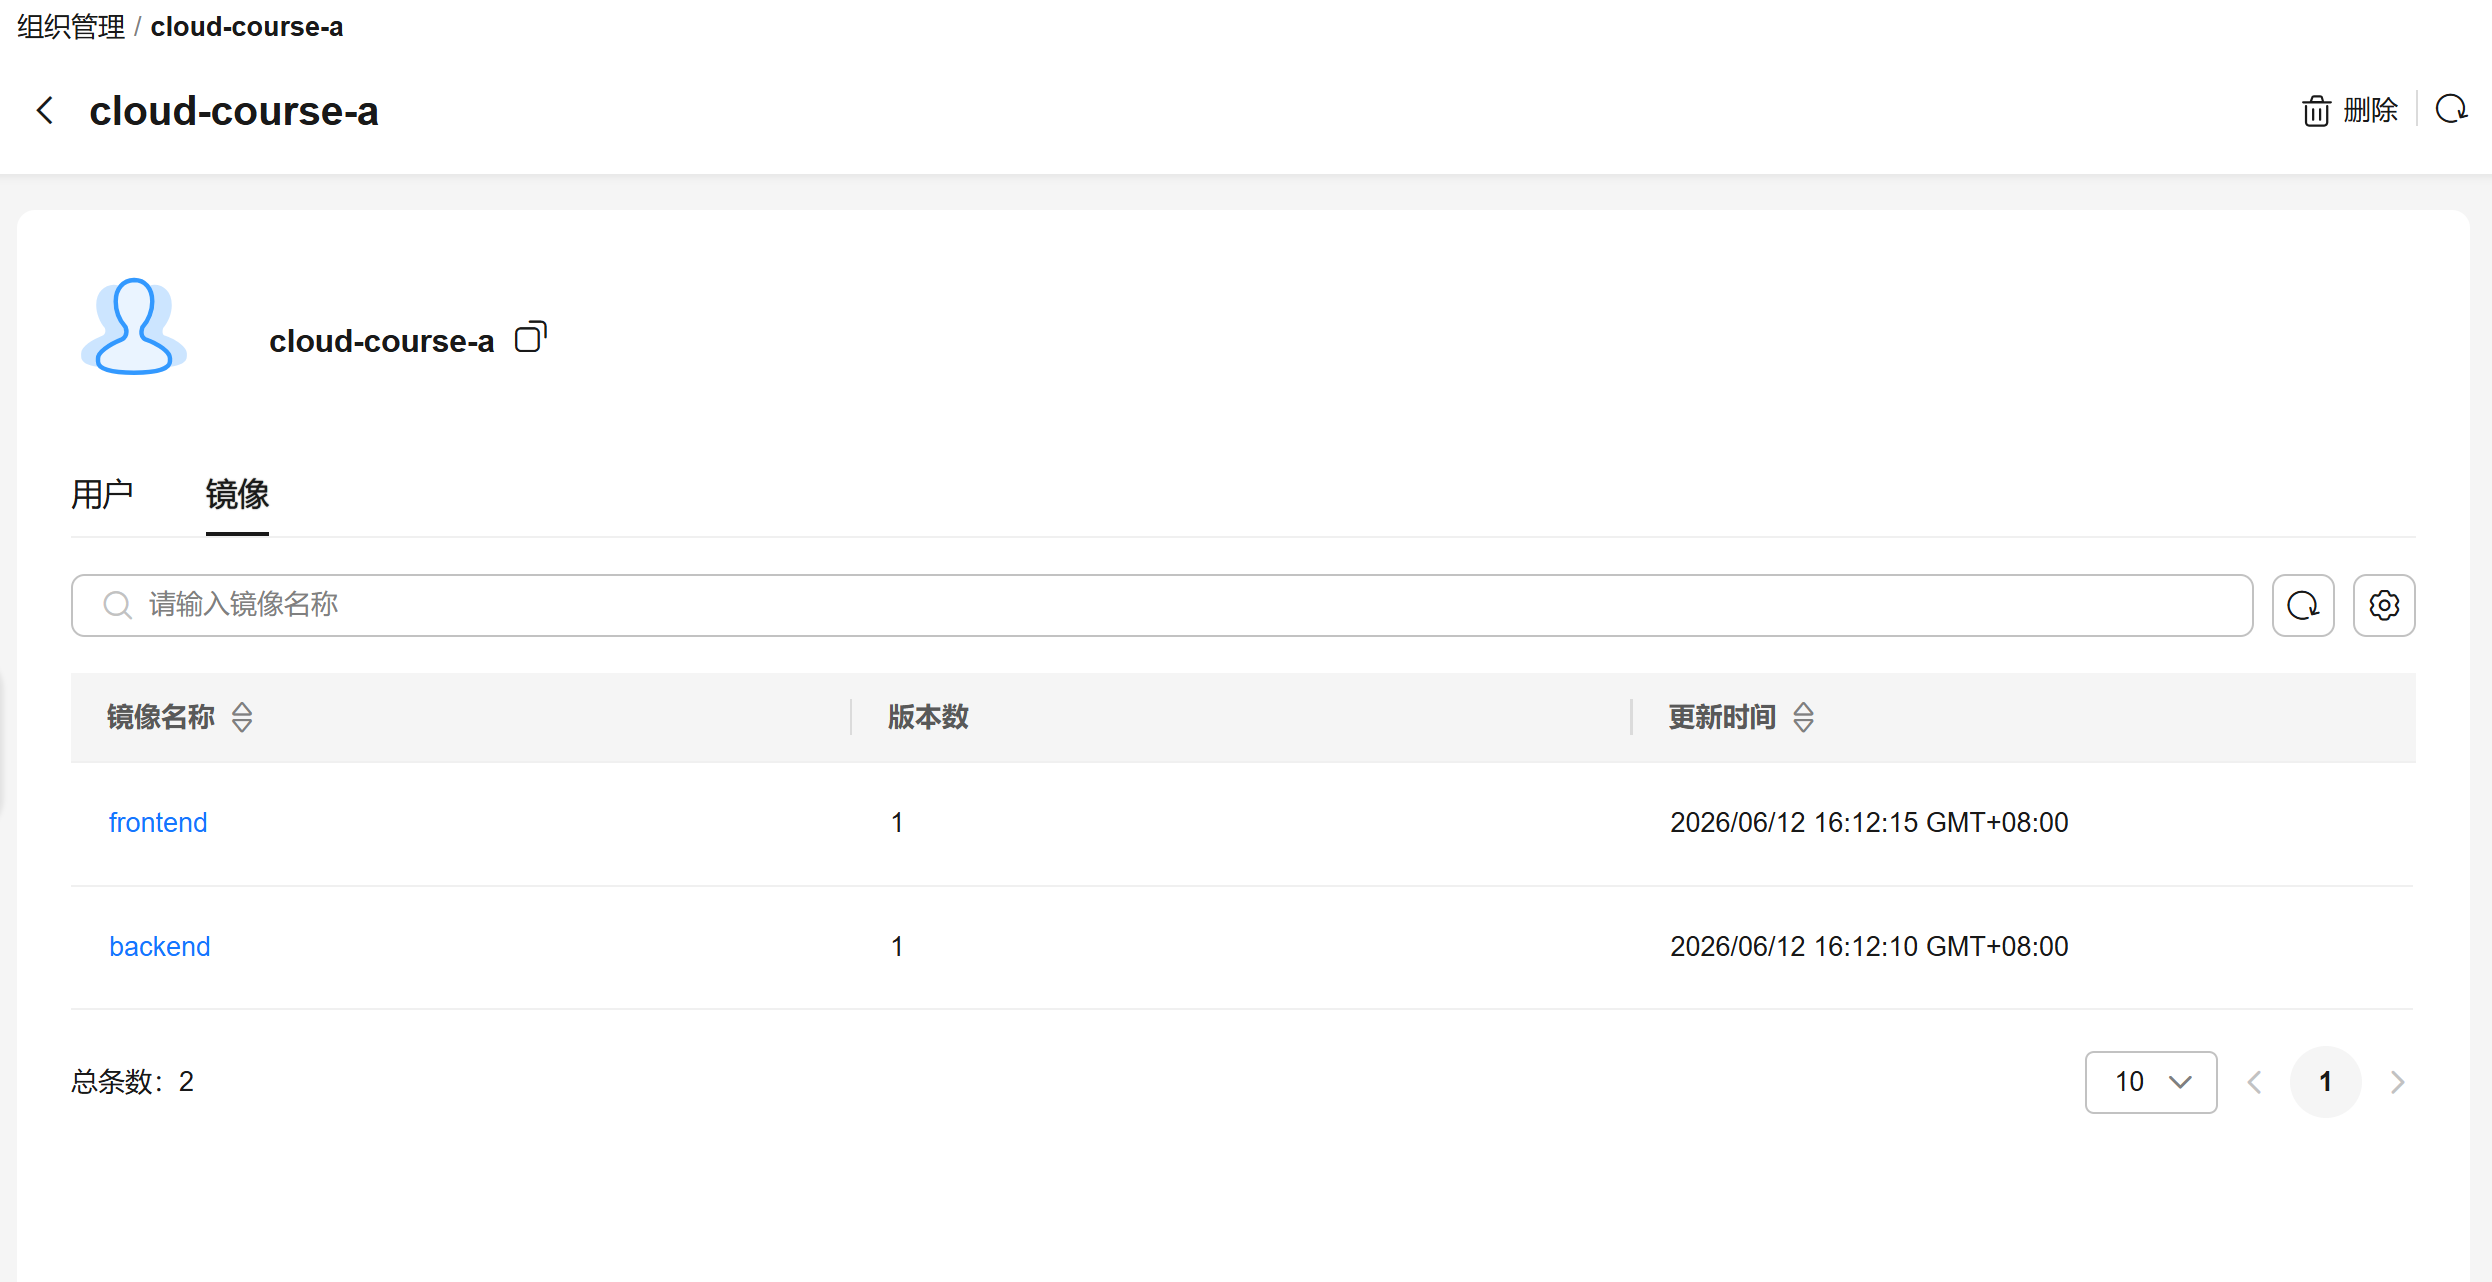
\includegraphics[width=0.92\textwidth]{assets/report_figures/env/env-swr-images.png}
  \caption{SWR 中 backend 与 frontend 镜像确认截图}
  \label{fig:env-swr-images}
\end{figure}

图 \ref{fig:env-swr-images} 中可以看到，郑瑞璟的 SWR 组织下已经有 \texttt{backend} 和 \texttt{frontend} 两个镜像，标签均为 \texttt{v1}。后续 CCE 部署引用的就是这里的镜像地址；如果私有镜像拉取失败，则需要在 Deployment 中配合 \texttt{imagePullSecrets} 处理鉴权问题。

\subsubsection{CCE集群配置}

CCE 是第一部分云计算平台搭建的核心服务。项目创建的是 CCE Standard 集群，集群名称为 \texttt{cloud-course-cce}，区域为华北-北京四，Kubernetes 版本为 v1.34，满足任务书中“集群版本不低于 1.27”的要求。网络方面，集群绑定 VPC \texttt{cloud-course-vpc}，网段为 \texttt{192.168.0.0/16}；子网名称为 \texttt{cloud-course-subnet}，网段为 \texttt{192.168.0.0/24}。节点方面，集群创建 2 个 Worker 节点，节点规格为 \texttt{c9.large.2}，即 2 vCPU / 4 GiB，操作系统为 Ubuntu 22.04.5 LTS，容器运行时为 containerd。

\begin{figure}[H]
  \centering
  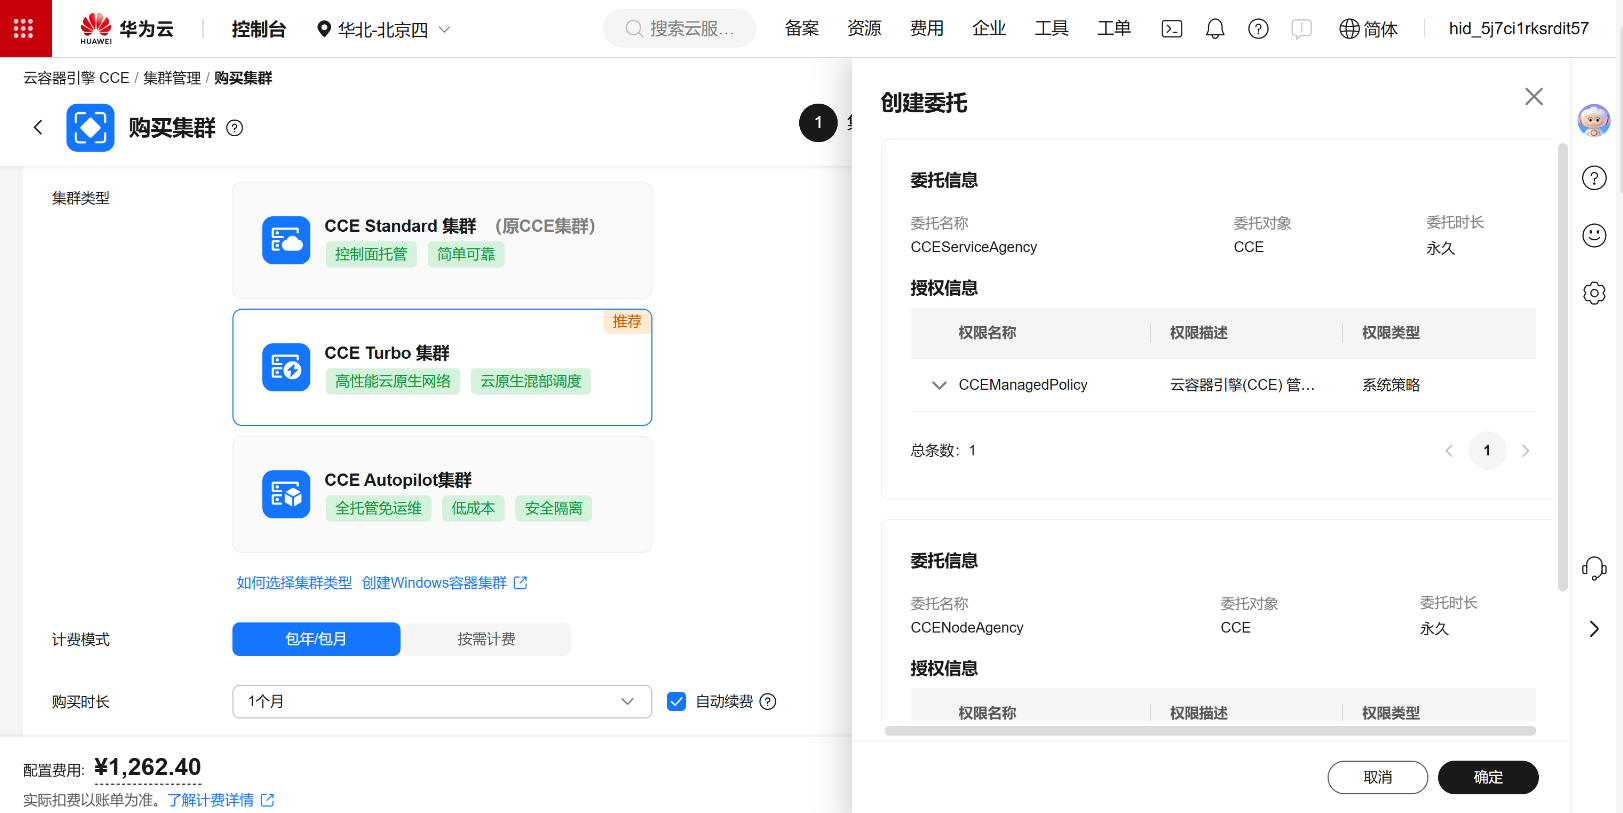
\includegraphics[width=0.92\textwidth]{assets/report_figures/t2/t2-01-cce-agency.png}
  \caption{首次使用 CCE 时创建服务委托截图}
  \label{fig:t2-cce-agency}
\end{figure}

图 \ref{fig:t2-cce-agency} 显示了首次使用 CCE 时创建服务委托的过程。CCE 作为托管 Kubernetes 服务，需要通过服务委托访问部分云资源，例如负载均衡、存储和网络资源。该步骤是后续自动创建或绑定云端资源的前置条件。

\begin{figure}[H]
  \centering
  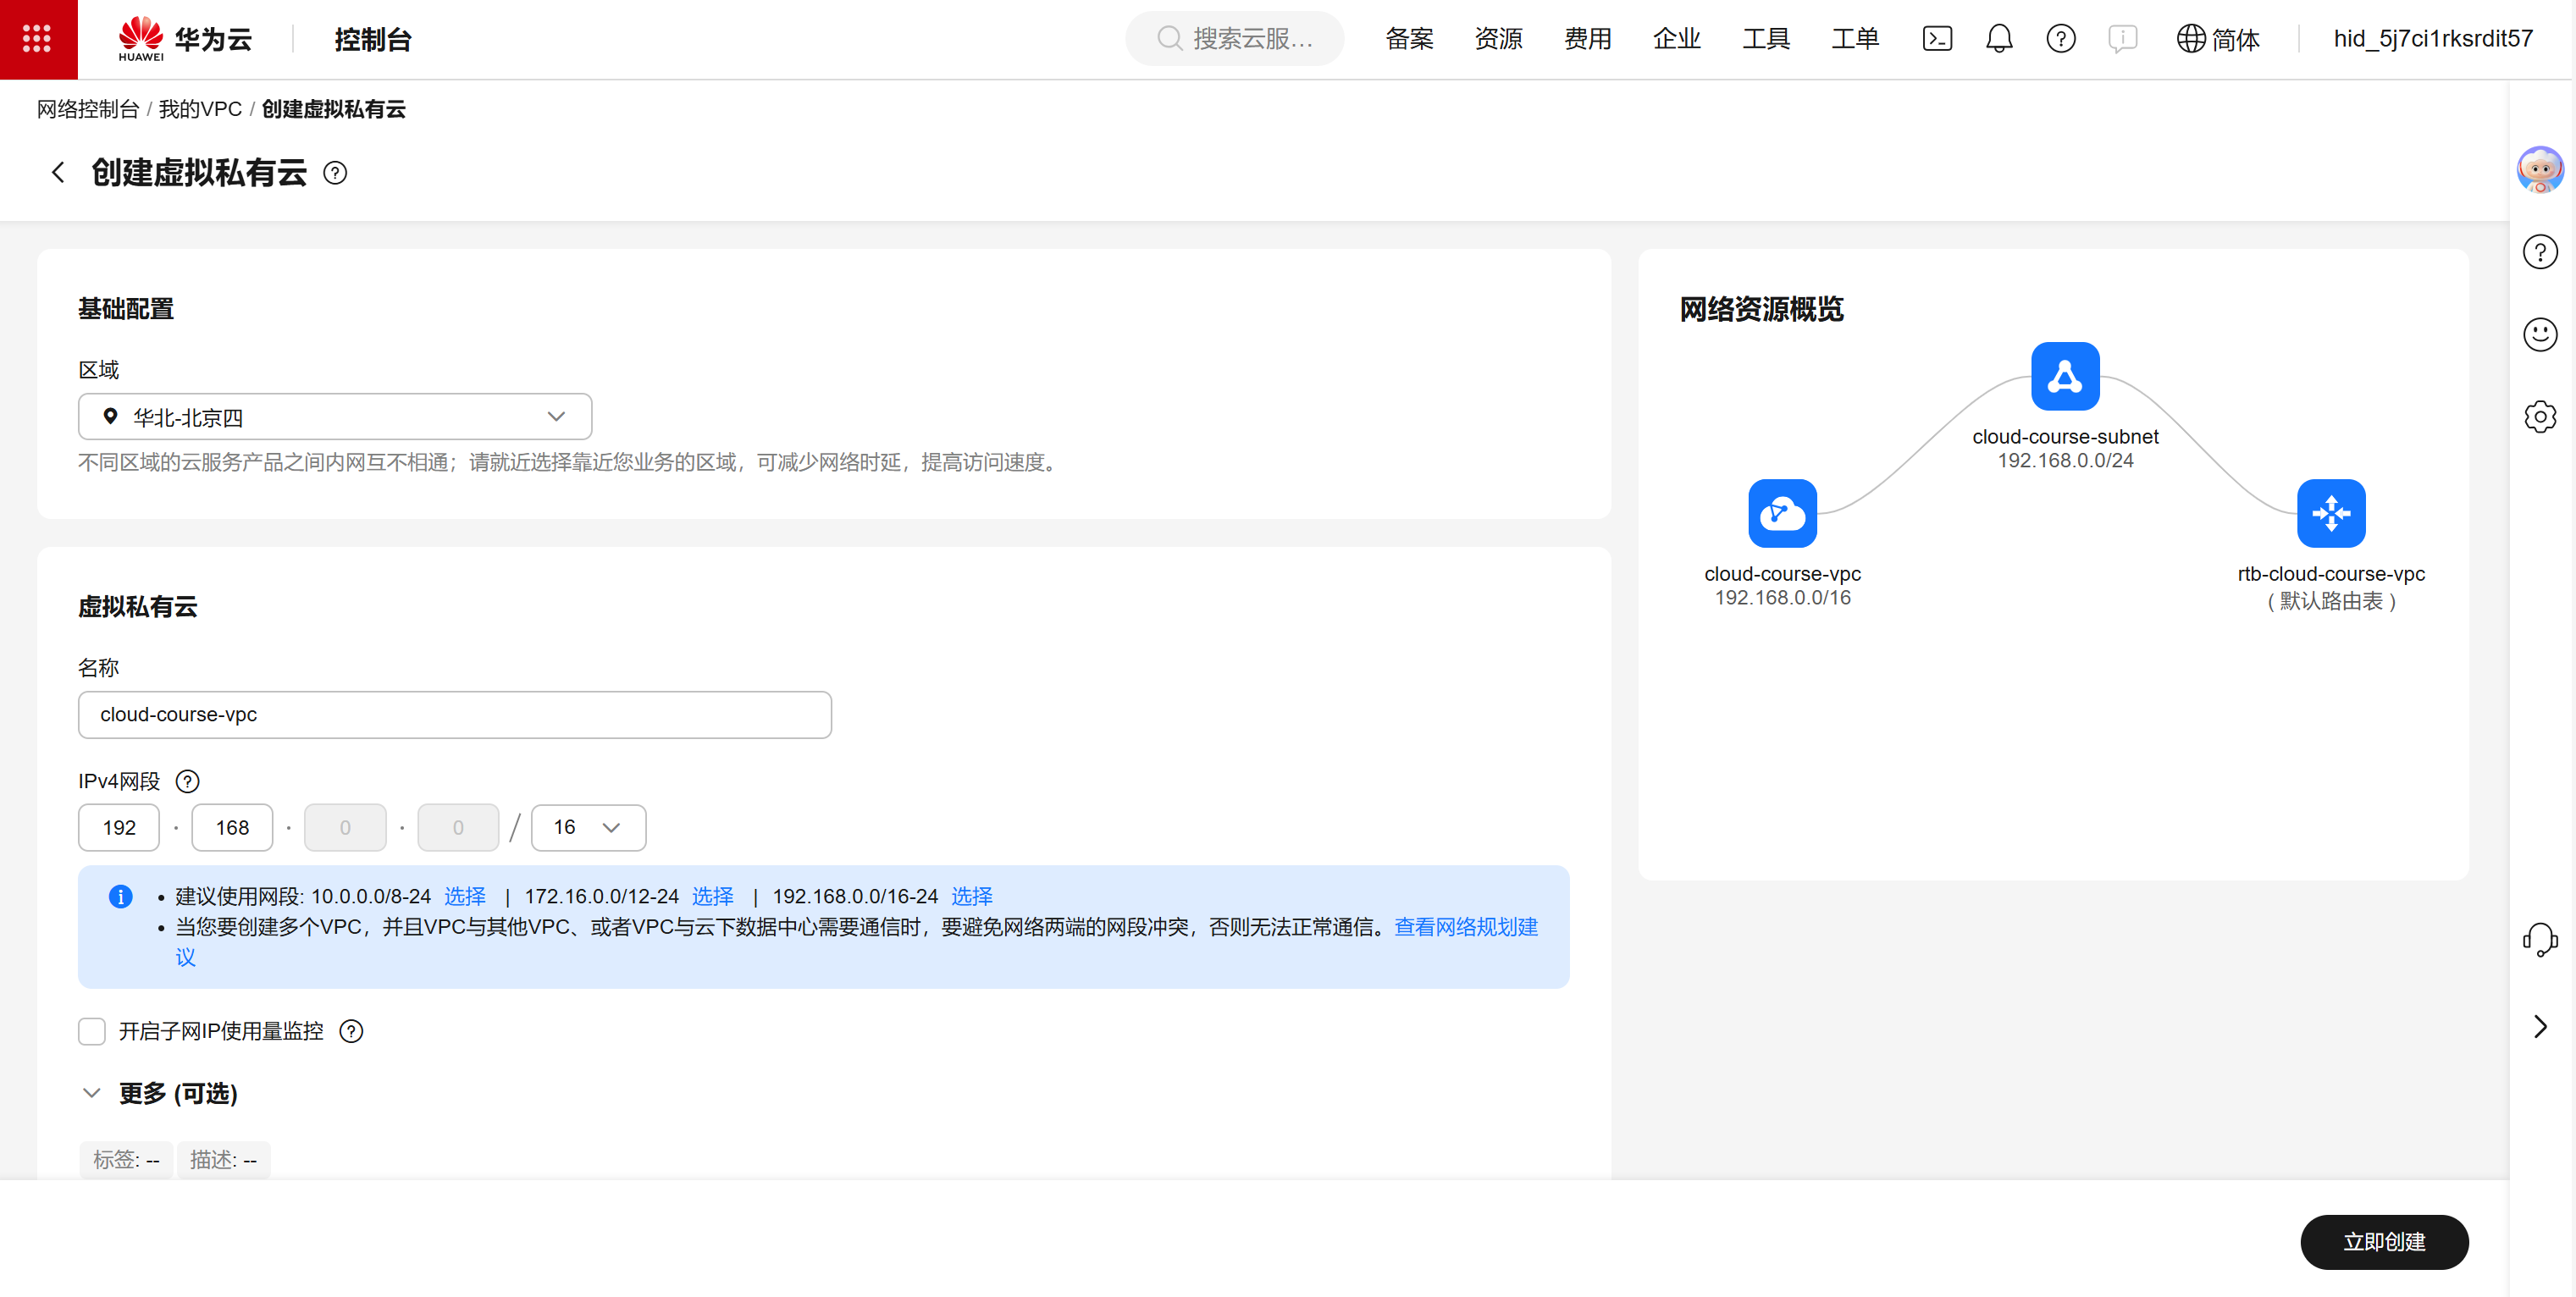
\includegraphics[width=0.92\textwidth]{assets/report_figures/t2/t2-02-vpc-subnet-config.png}
  \caption{创建 VPC 与子网配置页面截图}
  \label{fig:t2-vpc-subnet-config}
\end{figure}

图 \ref{fig:t2-vpc-subnet-config} 展示了 VPC 和子网的创建配置。VPC 为 CCE 节点、Pod 网络和云端负载均衡提供基础网络隔离环境，子网则决定 Worker 节点实际使用的内网地址范围。本项目使用统一命名的 \texttt{cloud-course-vpc} 和 \texttt{cloud-course-subnet}，便于后续资源定位和排错。

\begin{figure}[H]
  \centering
  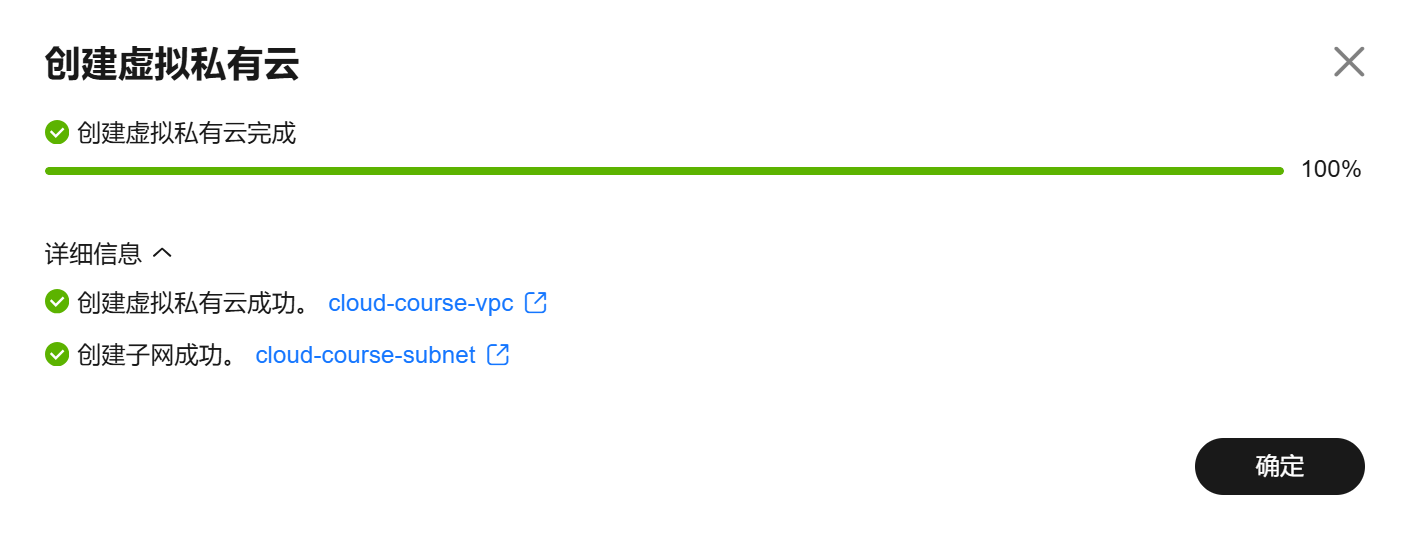
\includegraphics[width=0.92\textwidth]{assets/report_figures/t2/t2-03-vpc-subnet-created.png}
  \caption{VPC 与子网创建成功截图}
  \label{fig:t2-vpc-subnet-created}
\end{figure}

图 \ref{fig:t2-vpc-subnet-created} 表明 VPC 和子网已经创建完成。该结果说明 CCE 集群创建前的网络基础资源已经就绪，后续 Worker 节点可以加入该网络并获得内网 IP。

\begin{figure}[H]
  \centering
  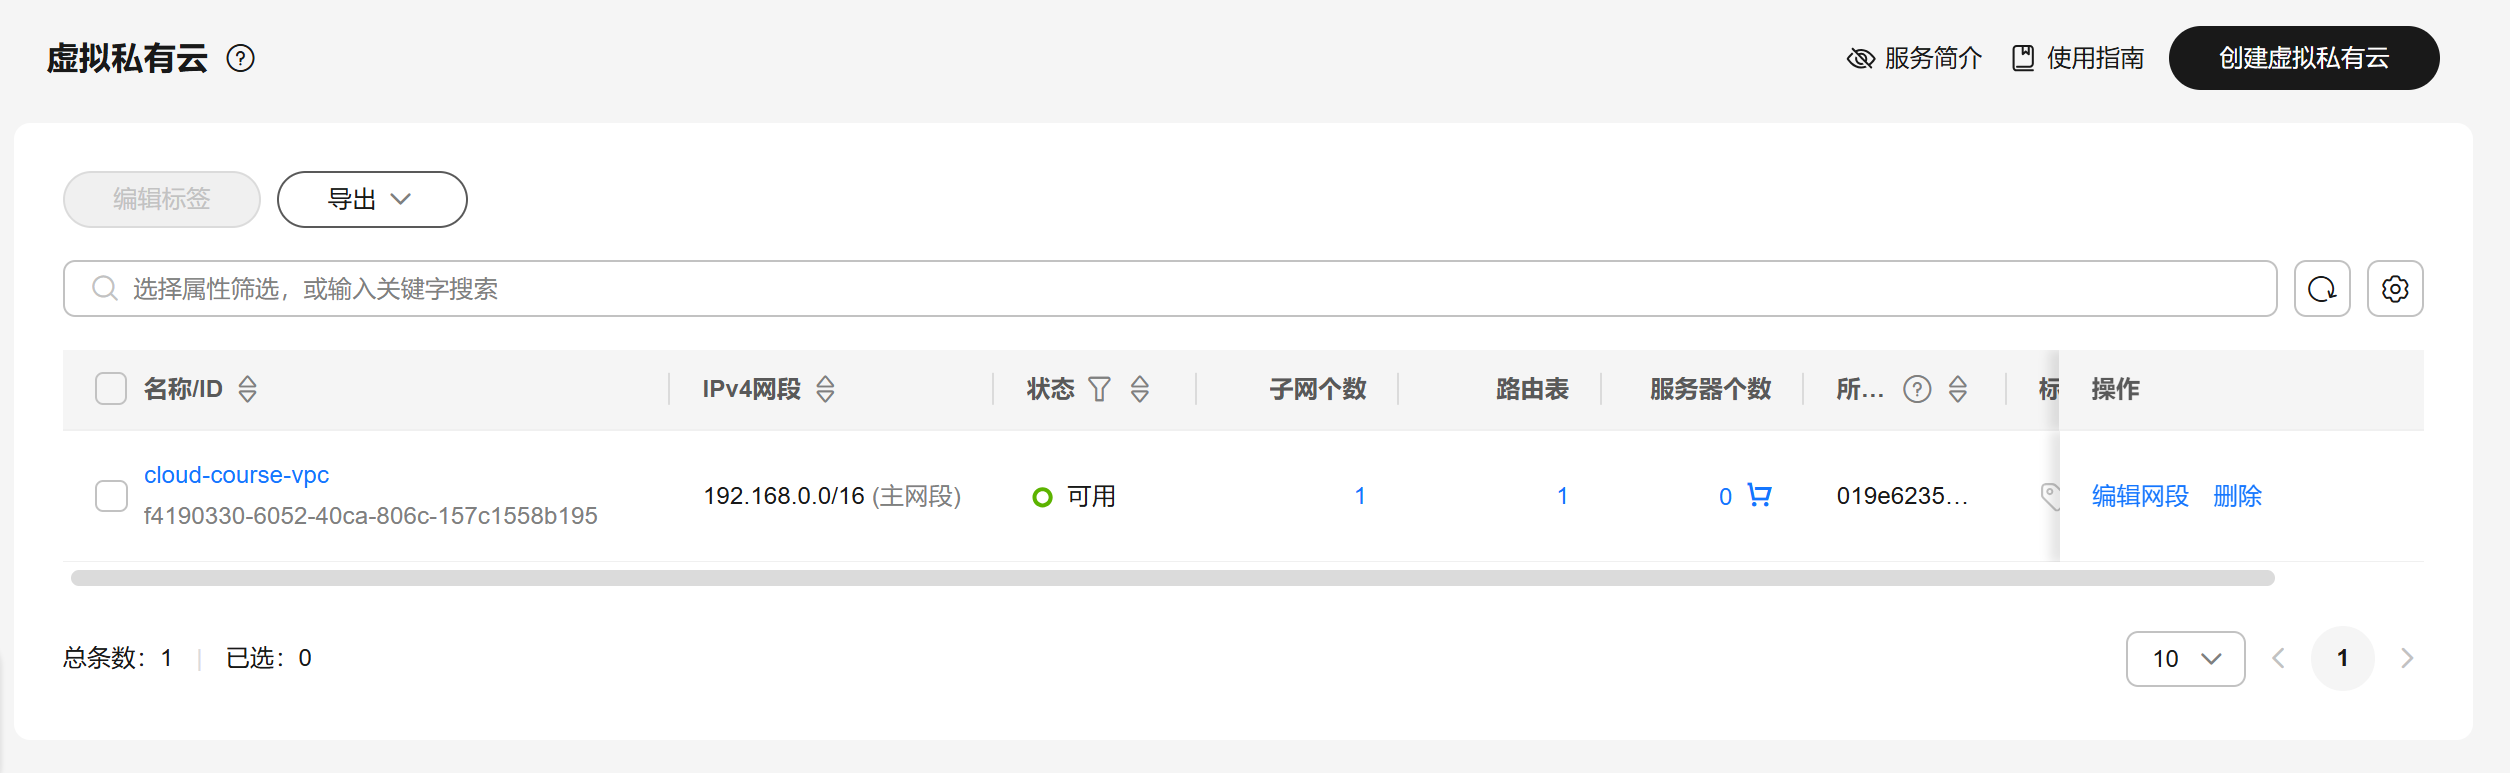
\includegraphics[width=0.92\textwidth]{assets/report_figures/t2/t2-04-vpc-list.png}
  \caption{VPC 列表中 cloud-course-vpc 状态可用截图}
  \label{fig:t2-vpc-list}
\end{figure}

图 \ref{fig:t2-vpc-list} 中，\texttt{cloud-course-vpc} 已处于可用状态。

\begin{figure}[H]
  \centering
  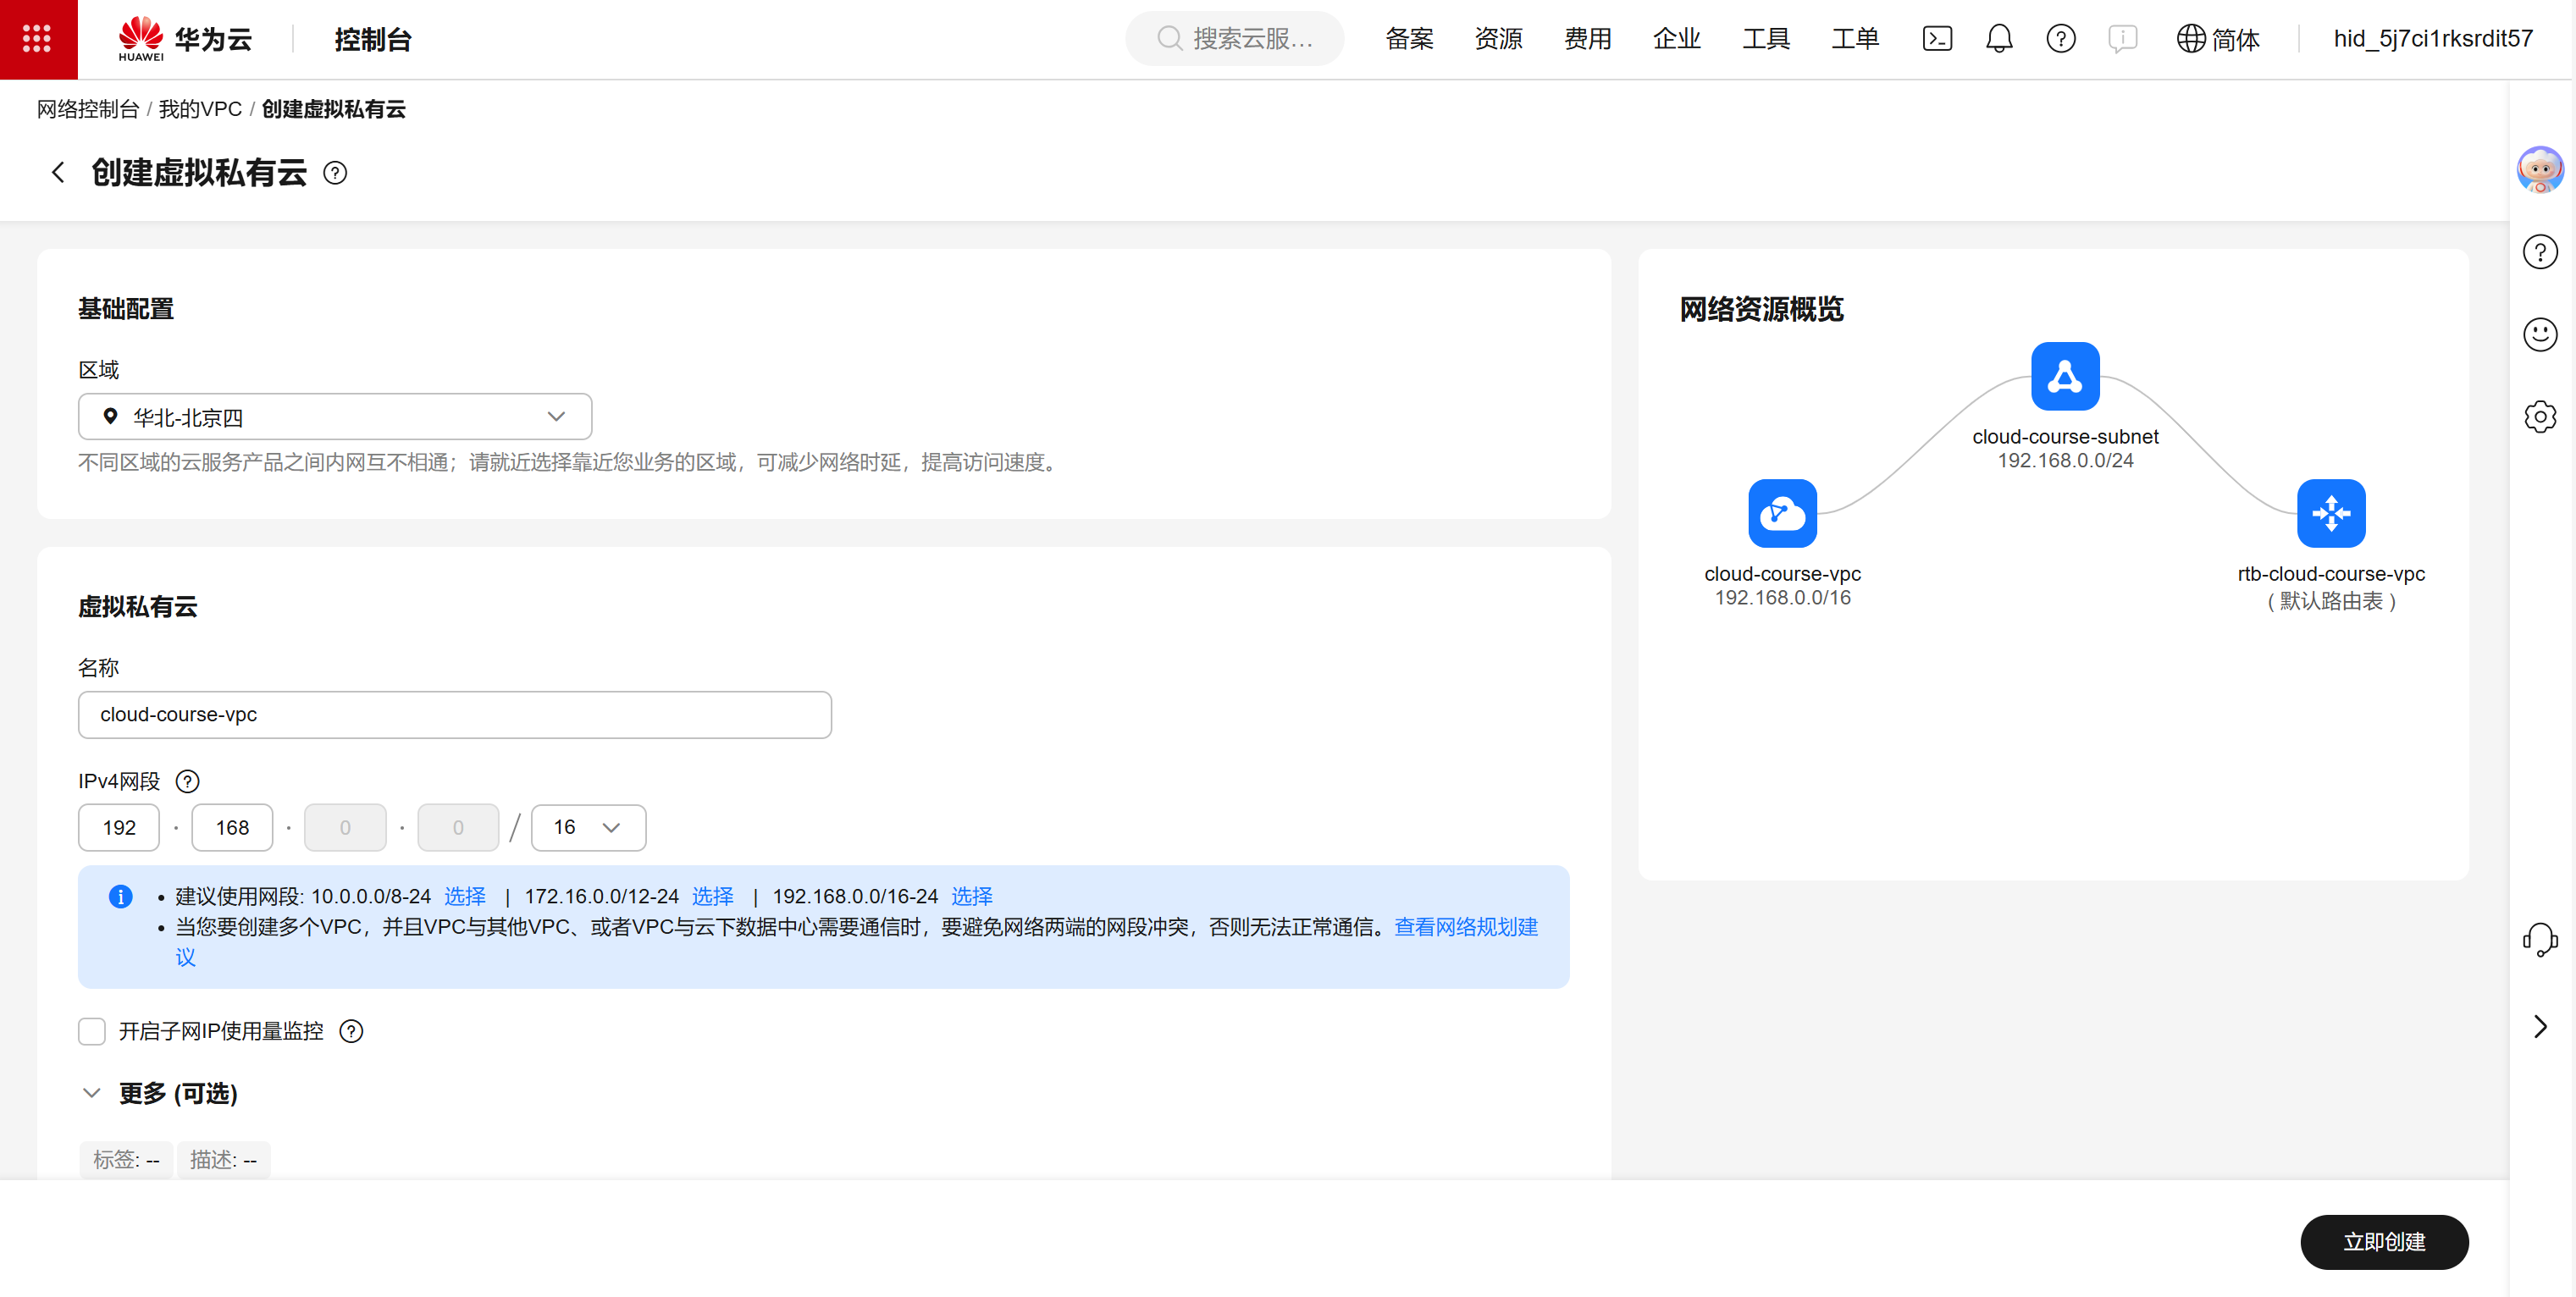
\includegraphics[width=0.92\textwidth]{assets/report_figures/t2/t2-05-cce-network-overview.png}
  \caption{CCE 集群网络配置总览截图}
  \label{fig:t2-cce-network-overview}
\end{figure}

图 \ref{fig:t2-cce-network-overview} 展示了 CCE 集群创建时的网络配置总览，页面中能看到集群绑定的 VPC、子网和容器网络配置。

\begin{figure}[H]
  \centering
  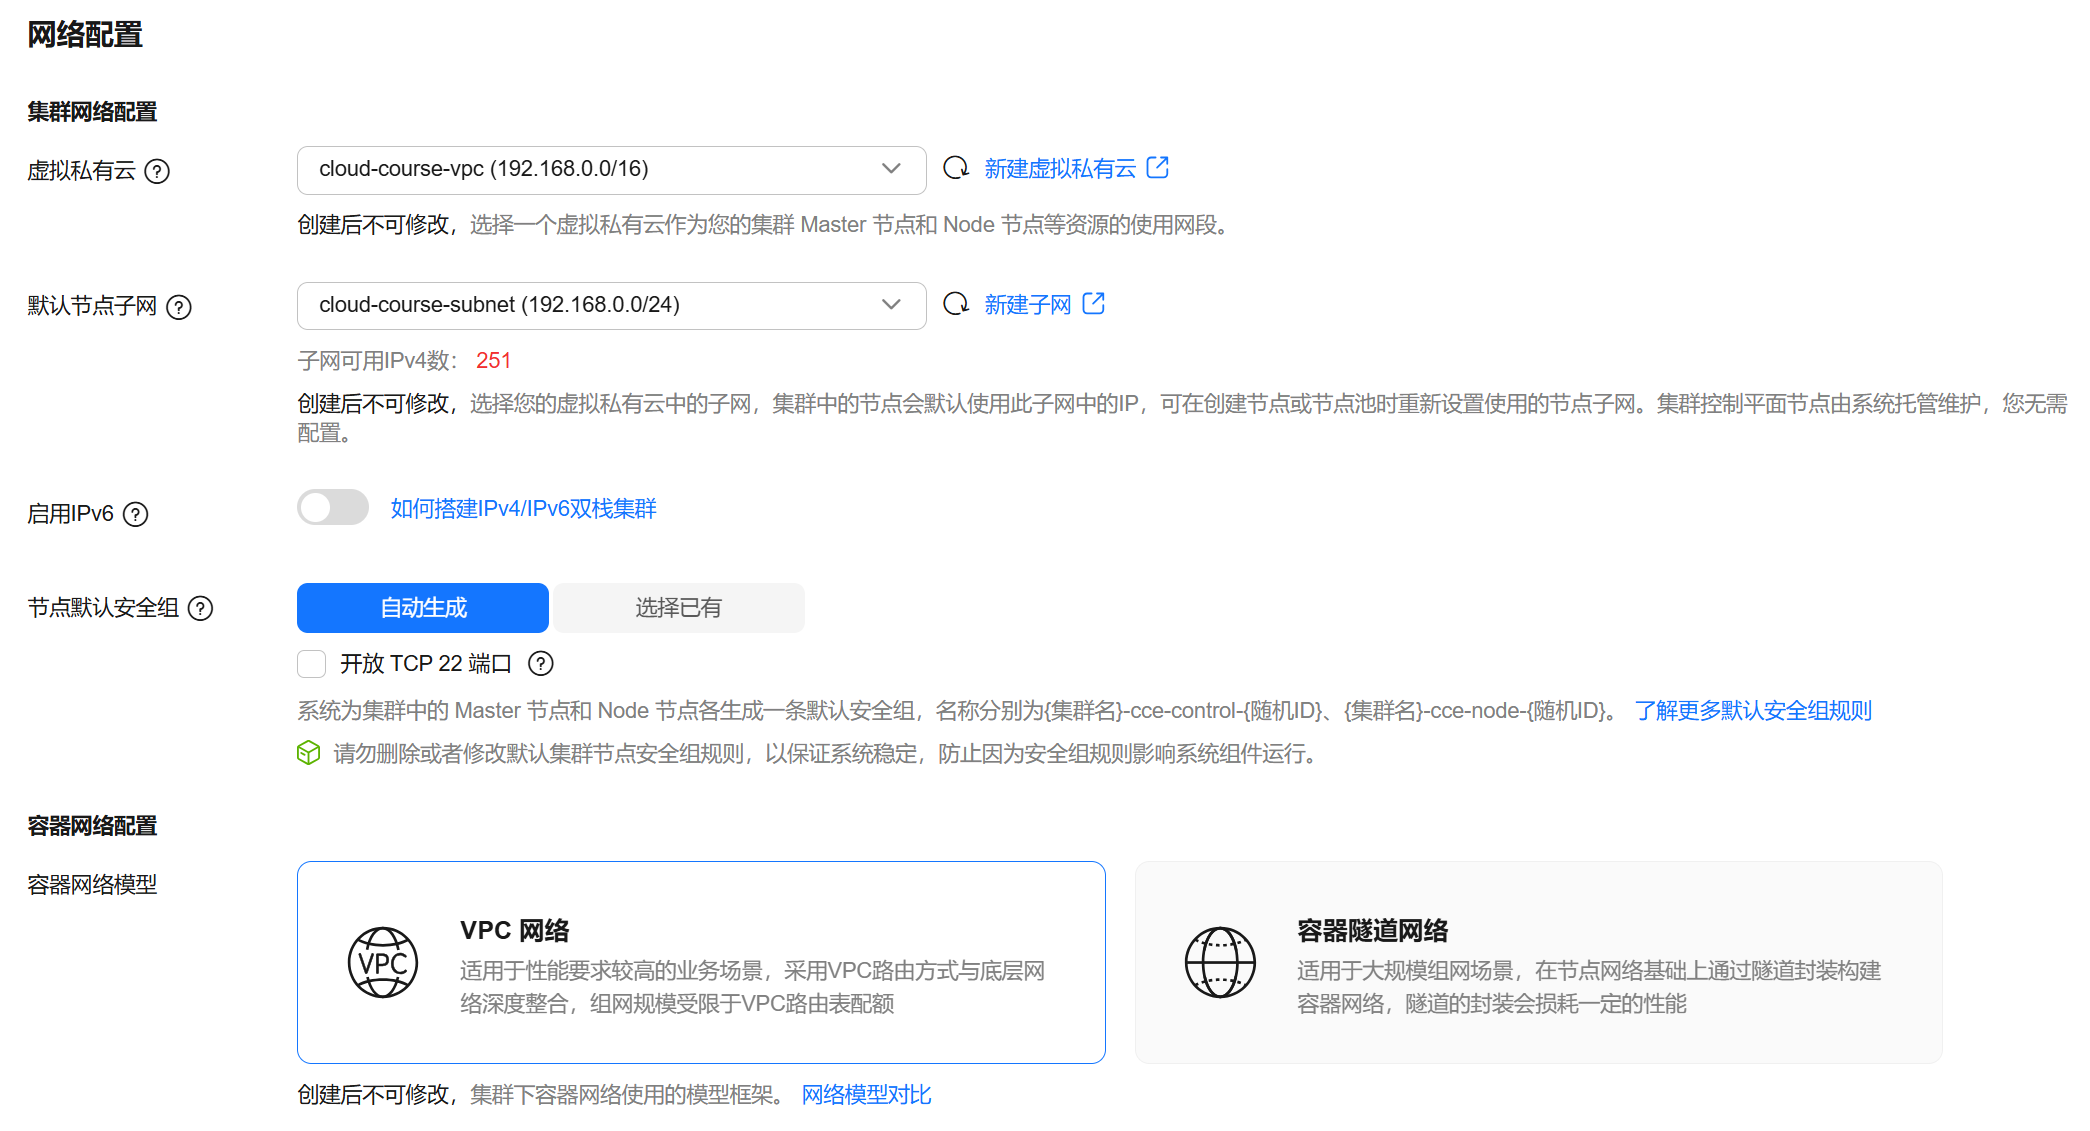
\includegraphics[width=0.92\textwidth]{assets/report_figures/t2/t2-06-cce-network-model.png}
  \caption{CCE 网络配置中 VPC、子网和容器网络模型截图}
  \label{fig:t2-cce-network-model}
\end{figure}

图 \ref{fig:t2-cce-network-model} 展示了 CCE 网络模型配置，可以看到集群使用的 VPC、子网和容器网络模型。

\begin{figure}[H]
  \centering
  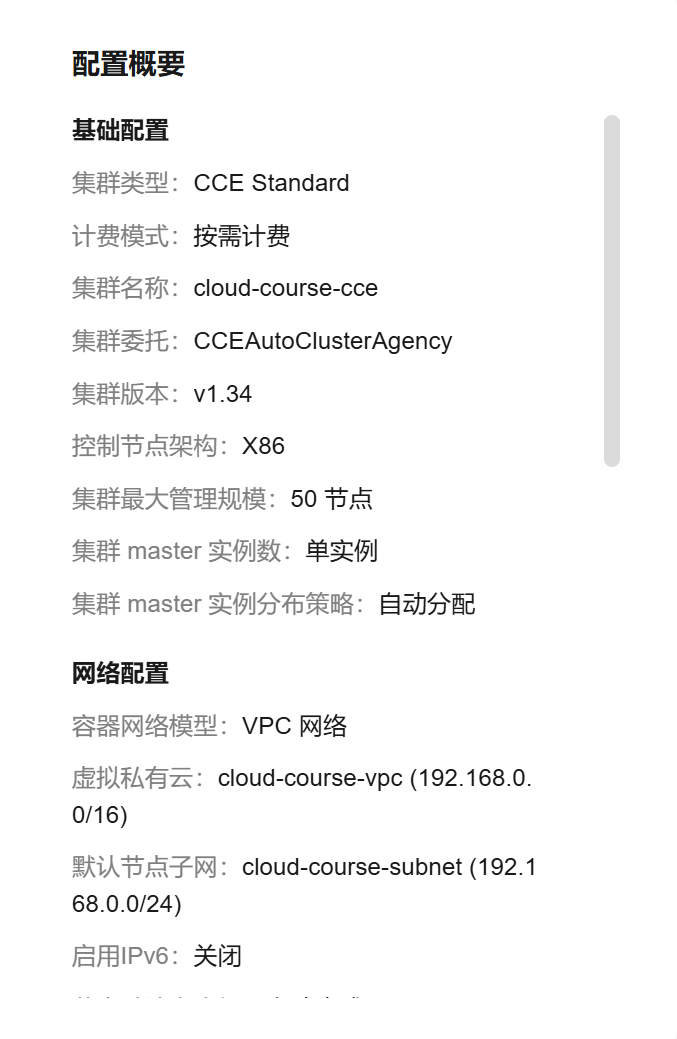
\includegraphics[width=0.68\textwidth]{assets/report_figures/t2/t2-07-cce-basic-summary.png}
  \caption{CCE 基础配置概要截图}
  \label{fig:t2-cce-basic-summary}
\end{figure}

图 \ref{fig:t2-cce-basic-summary} 中可以看到集群名称、集群类型和 Kubernetes 版本。

\begin{figure}[H]
  \centering
  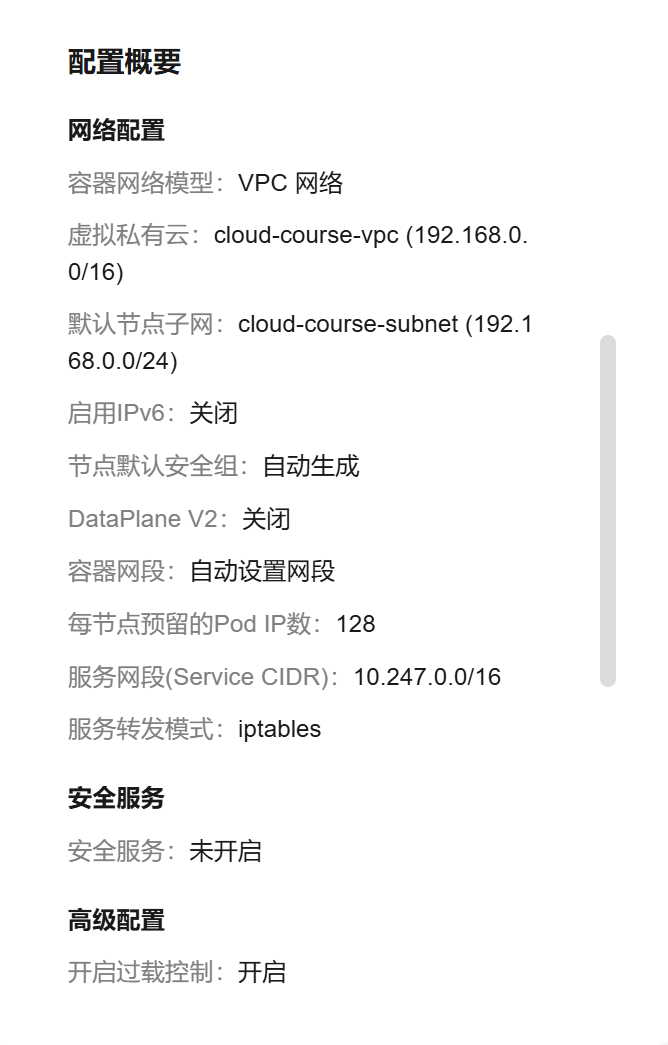
\includegraphics[width=0.55\textwidth]{assets/report_figures/t2/t2-09-cce-security-summary.png}
  \caption{CCE 网络与安全服务配置概要截图}
  \label{fig:t2-cce-security-summary}
\end{figure}

图 \ref{fig:t2-cce-security-summary} 展示了网络与安全服务配置，包括安全组和相关云服务选项。

\begin{figure}[H]
  \centering
  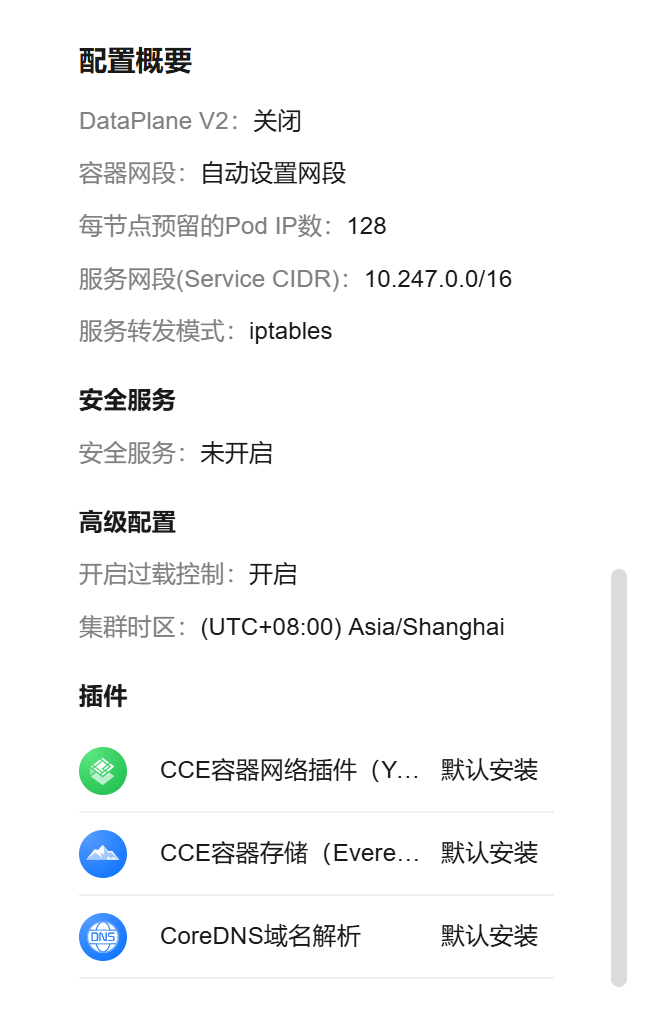
\includegraphics[width=0.55\textwidth]{assets/report_figures/t2/t2-10-cce-plugin-summary.png}
  \caption{CCE 网络与默认插件配置概要截图}
  \label{fig:t2-cce-plugin-summary}
\end{figure}

图 \ref{fig:t2-cce-plugin-summary} 展示了网络配置和默认插件配置。这里保留 CoreDNS、存储插件和容器网络插件，用于后续 Pod 通信、服务名解析和 PVC 挂载。

\begin{figure}[H]
  \centering
  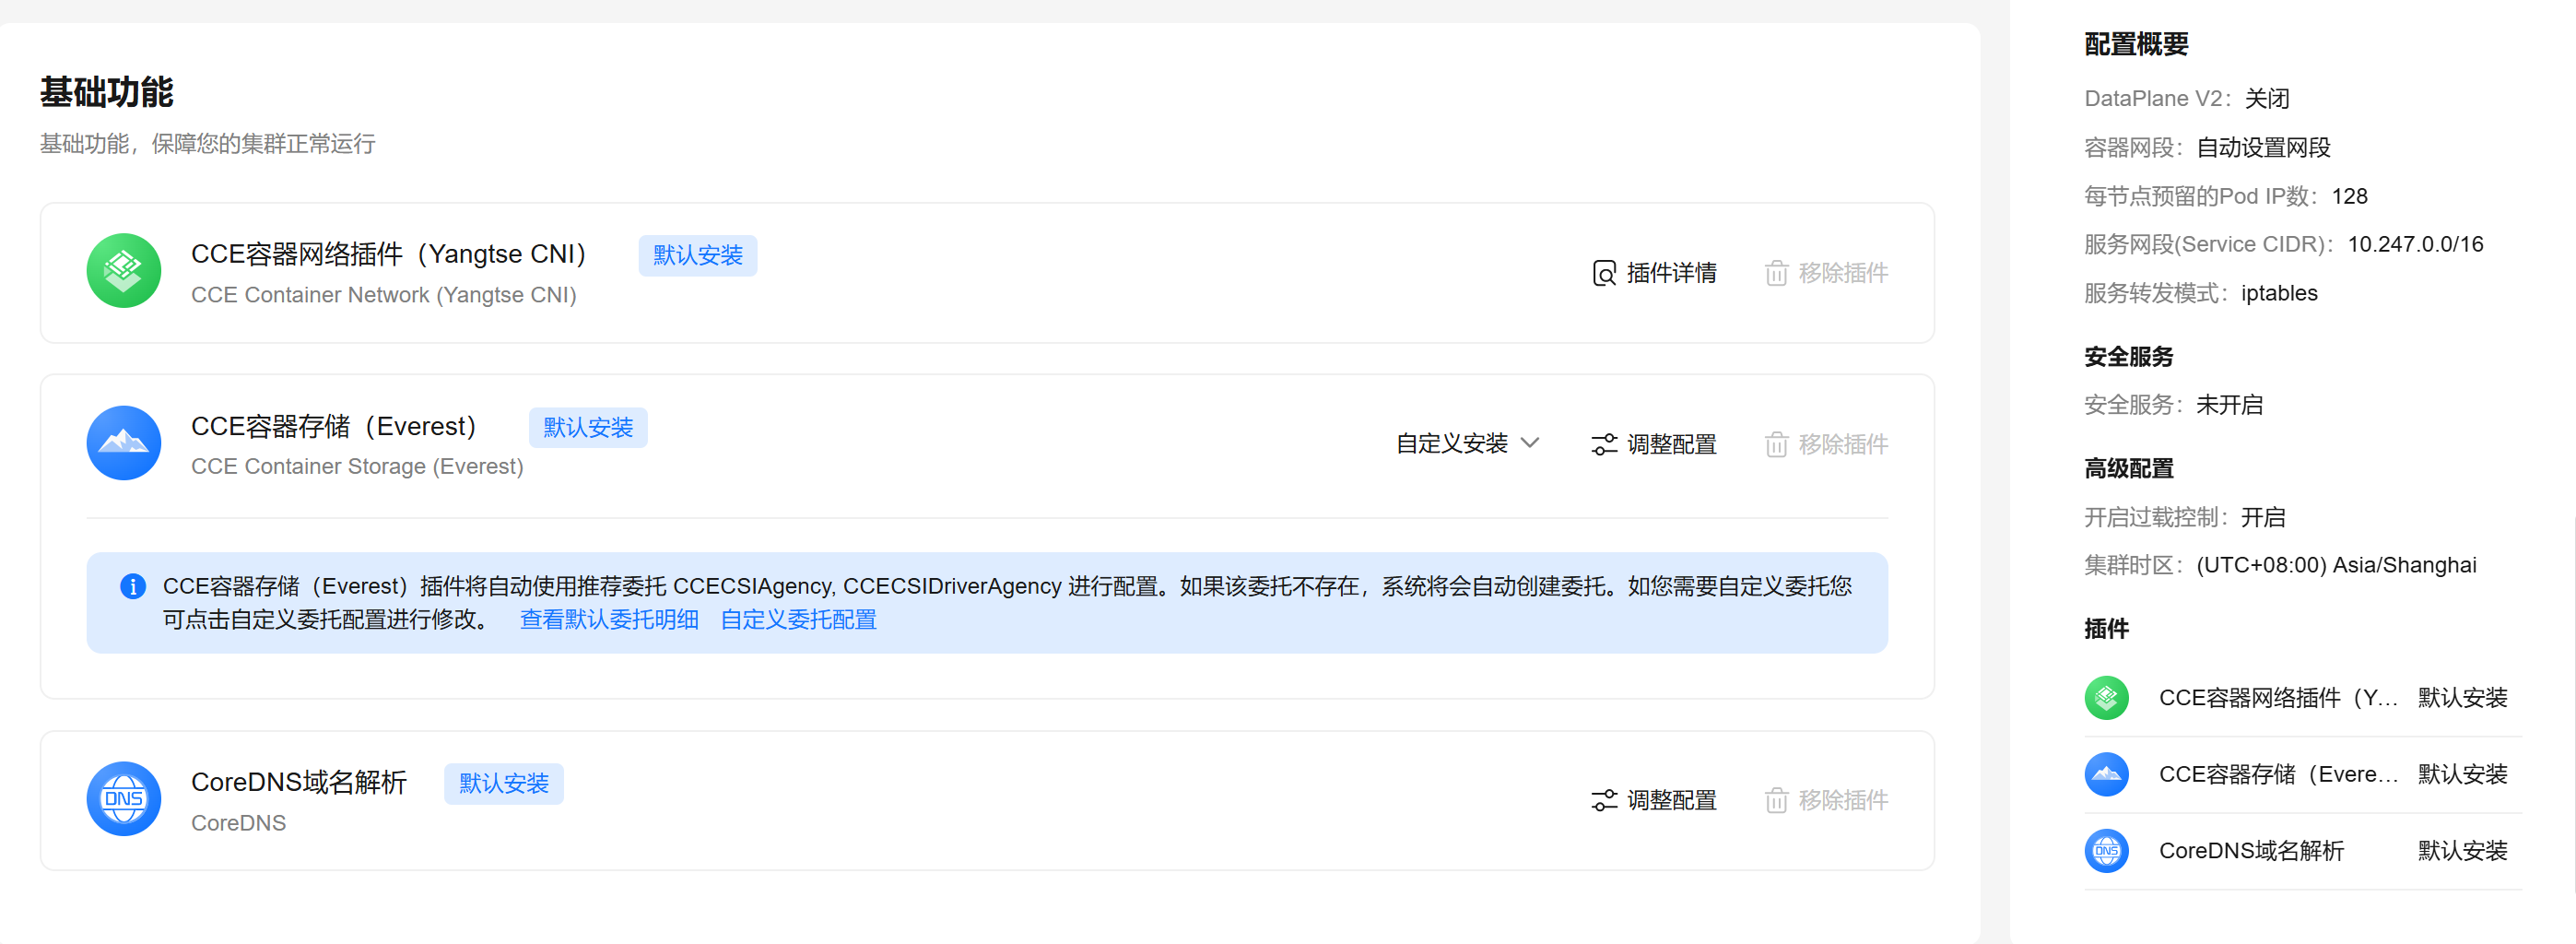
\includegraphics[width=0.92\textwidth]{assets/report_figures/t2/t2-11-cce-plugins.png}
  \caption{CCE 默认必要插件配置截图}
  \label{fig:t2-cce-plugins}
\end{figure}

图 \ref{fig:t2-cce-plugins} 展示了 CCE 集群创建时保留的默认必要插件。CoreDNS 用于集群内部服务名解析，Everest 存储插件用于后续 PVC 与云硬盘的对接，容器网络插件用于 Pod 网络通信。这些插件虽然不是业务应用代码的一部分，但它们决定了 Kubernetes 集群是否具备完整的基础能力。

\begin{figure}[H]
  \centering
  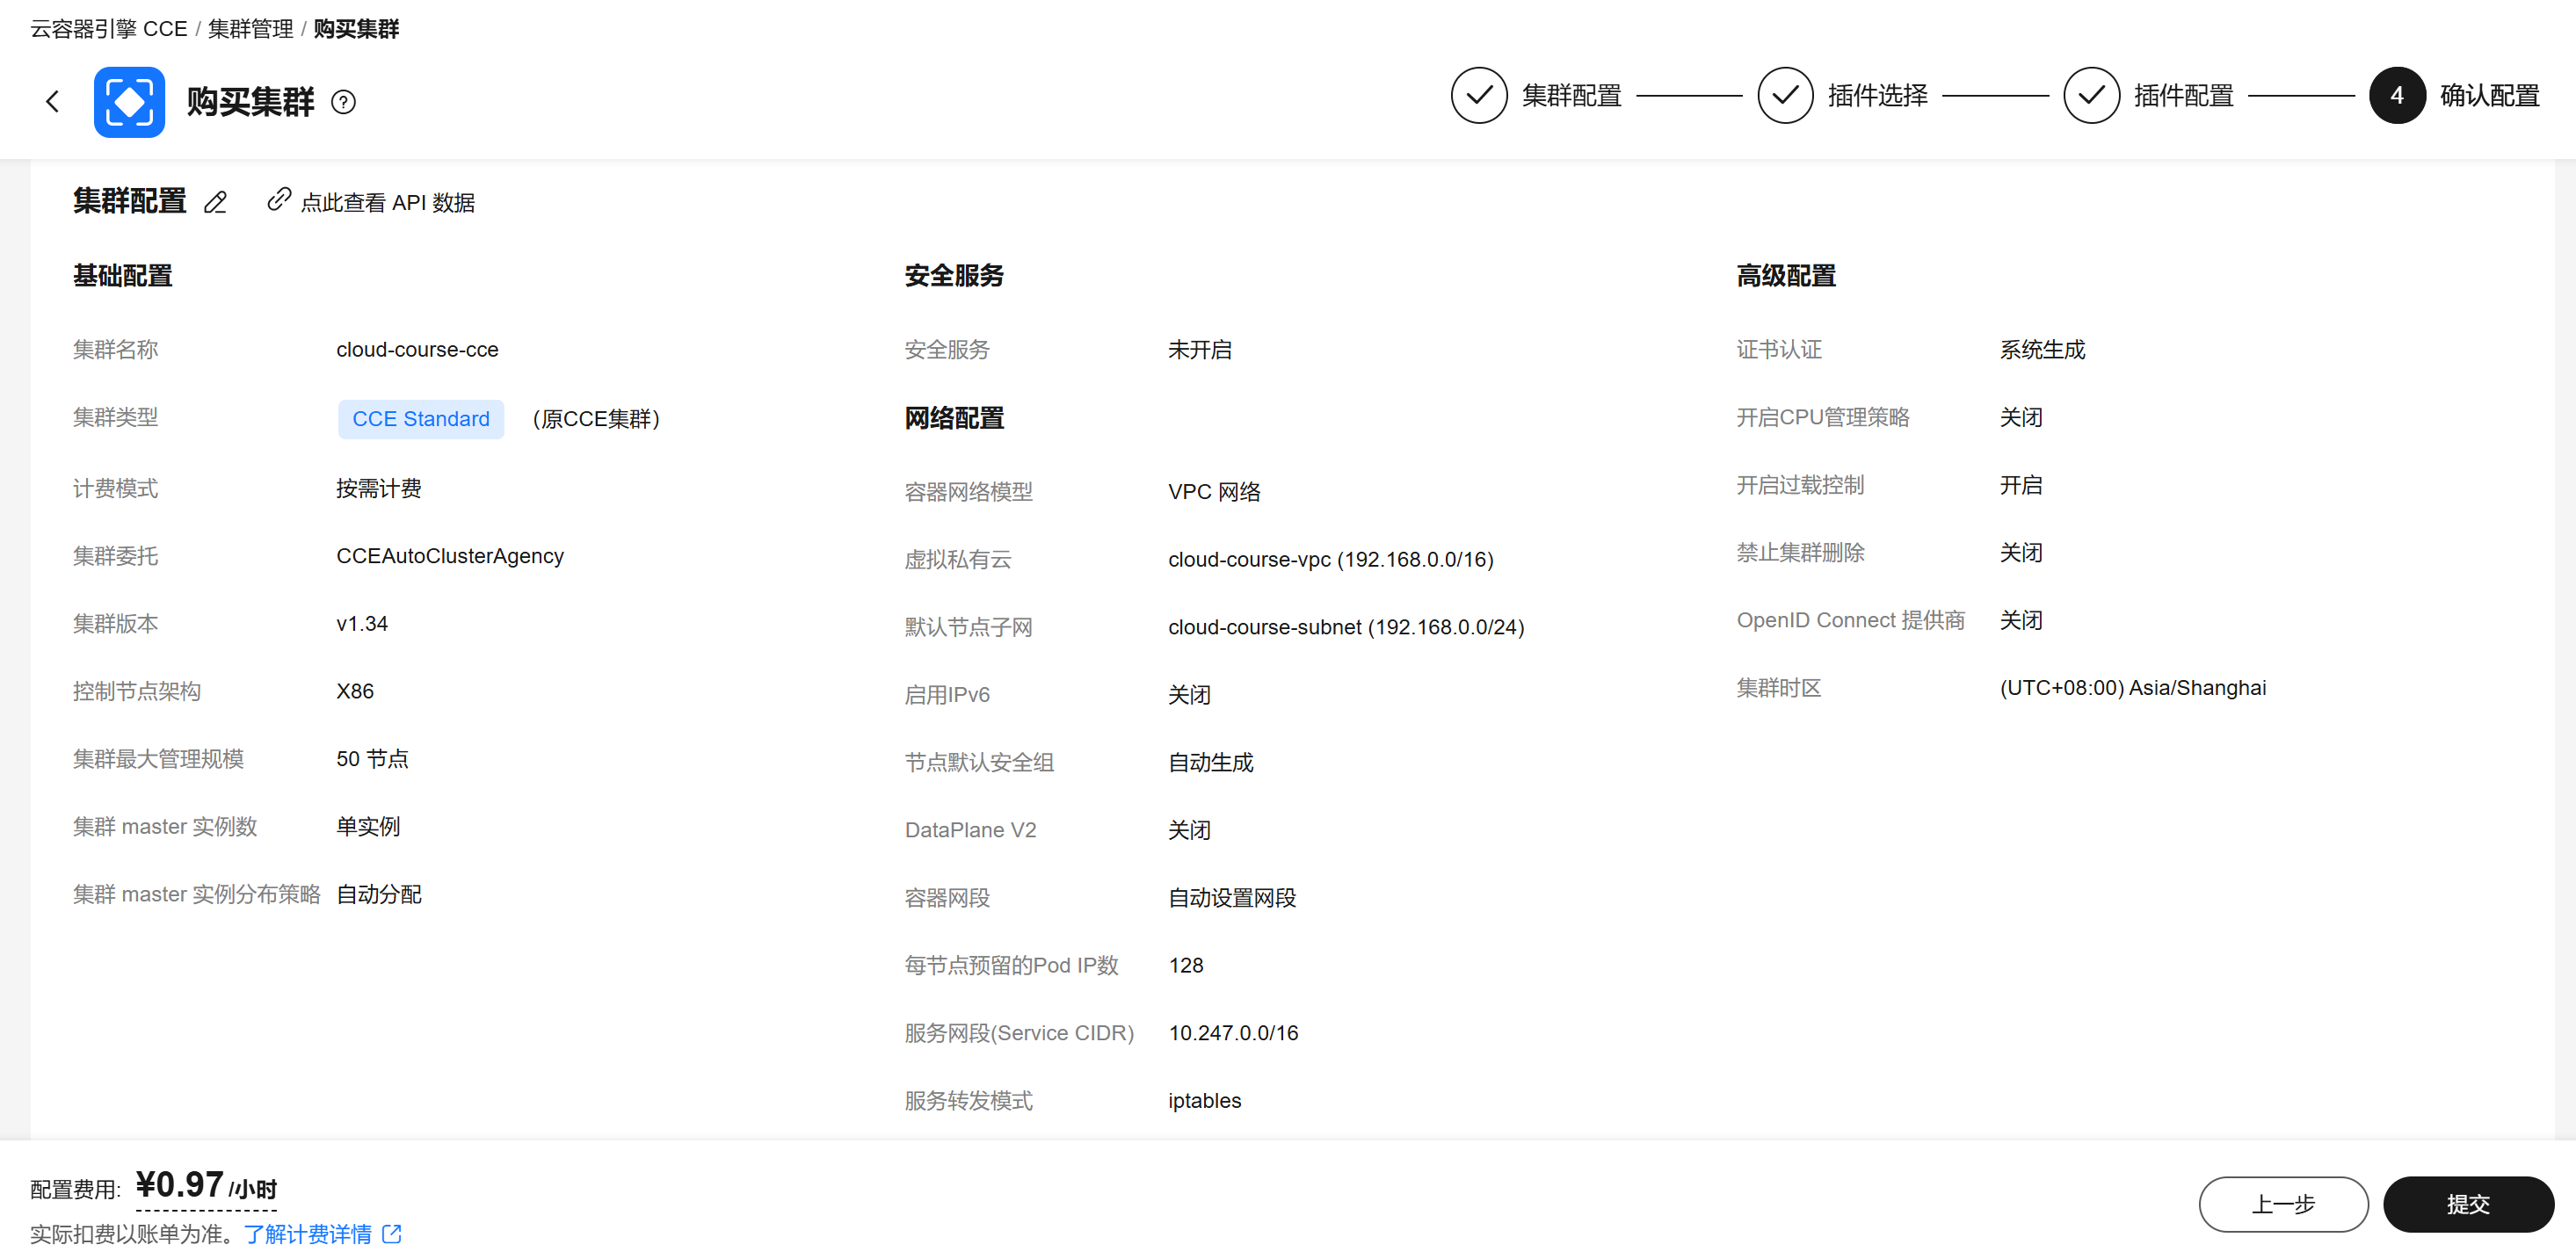
\includegraphics[width=0.80\textwidth]{assets/report_figures/t2/t2-12-cce-final-confirm.png}
  \caption{提交创建 CCE 集群前的最终配置确认截图}
  \label{fig:t2-cce-final-confirm}
\end{figure}

图 \ref{fig:t2-cce-final-confirm} 是提交创建 CCE 集群前的最终确认页面，用来核对集群名称、版本、节点和网络等参数。

\begin{figure}[H]
  \centering
  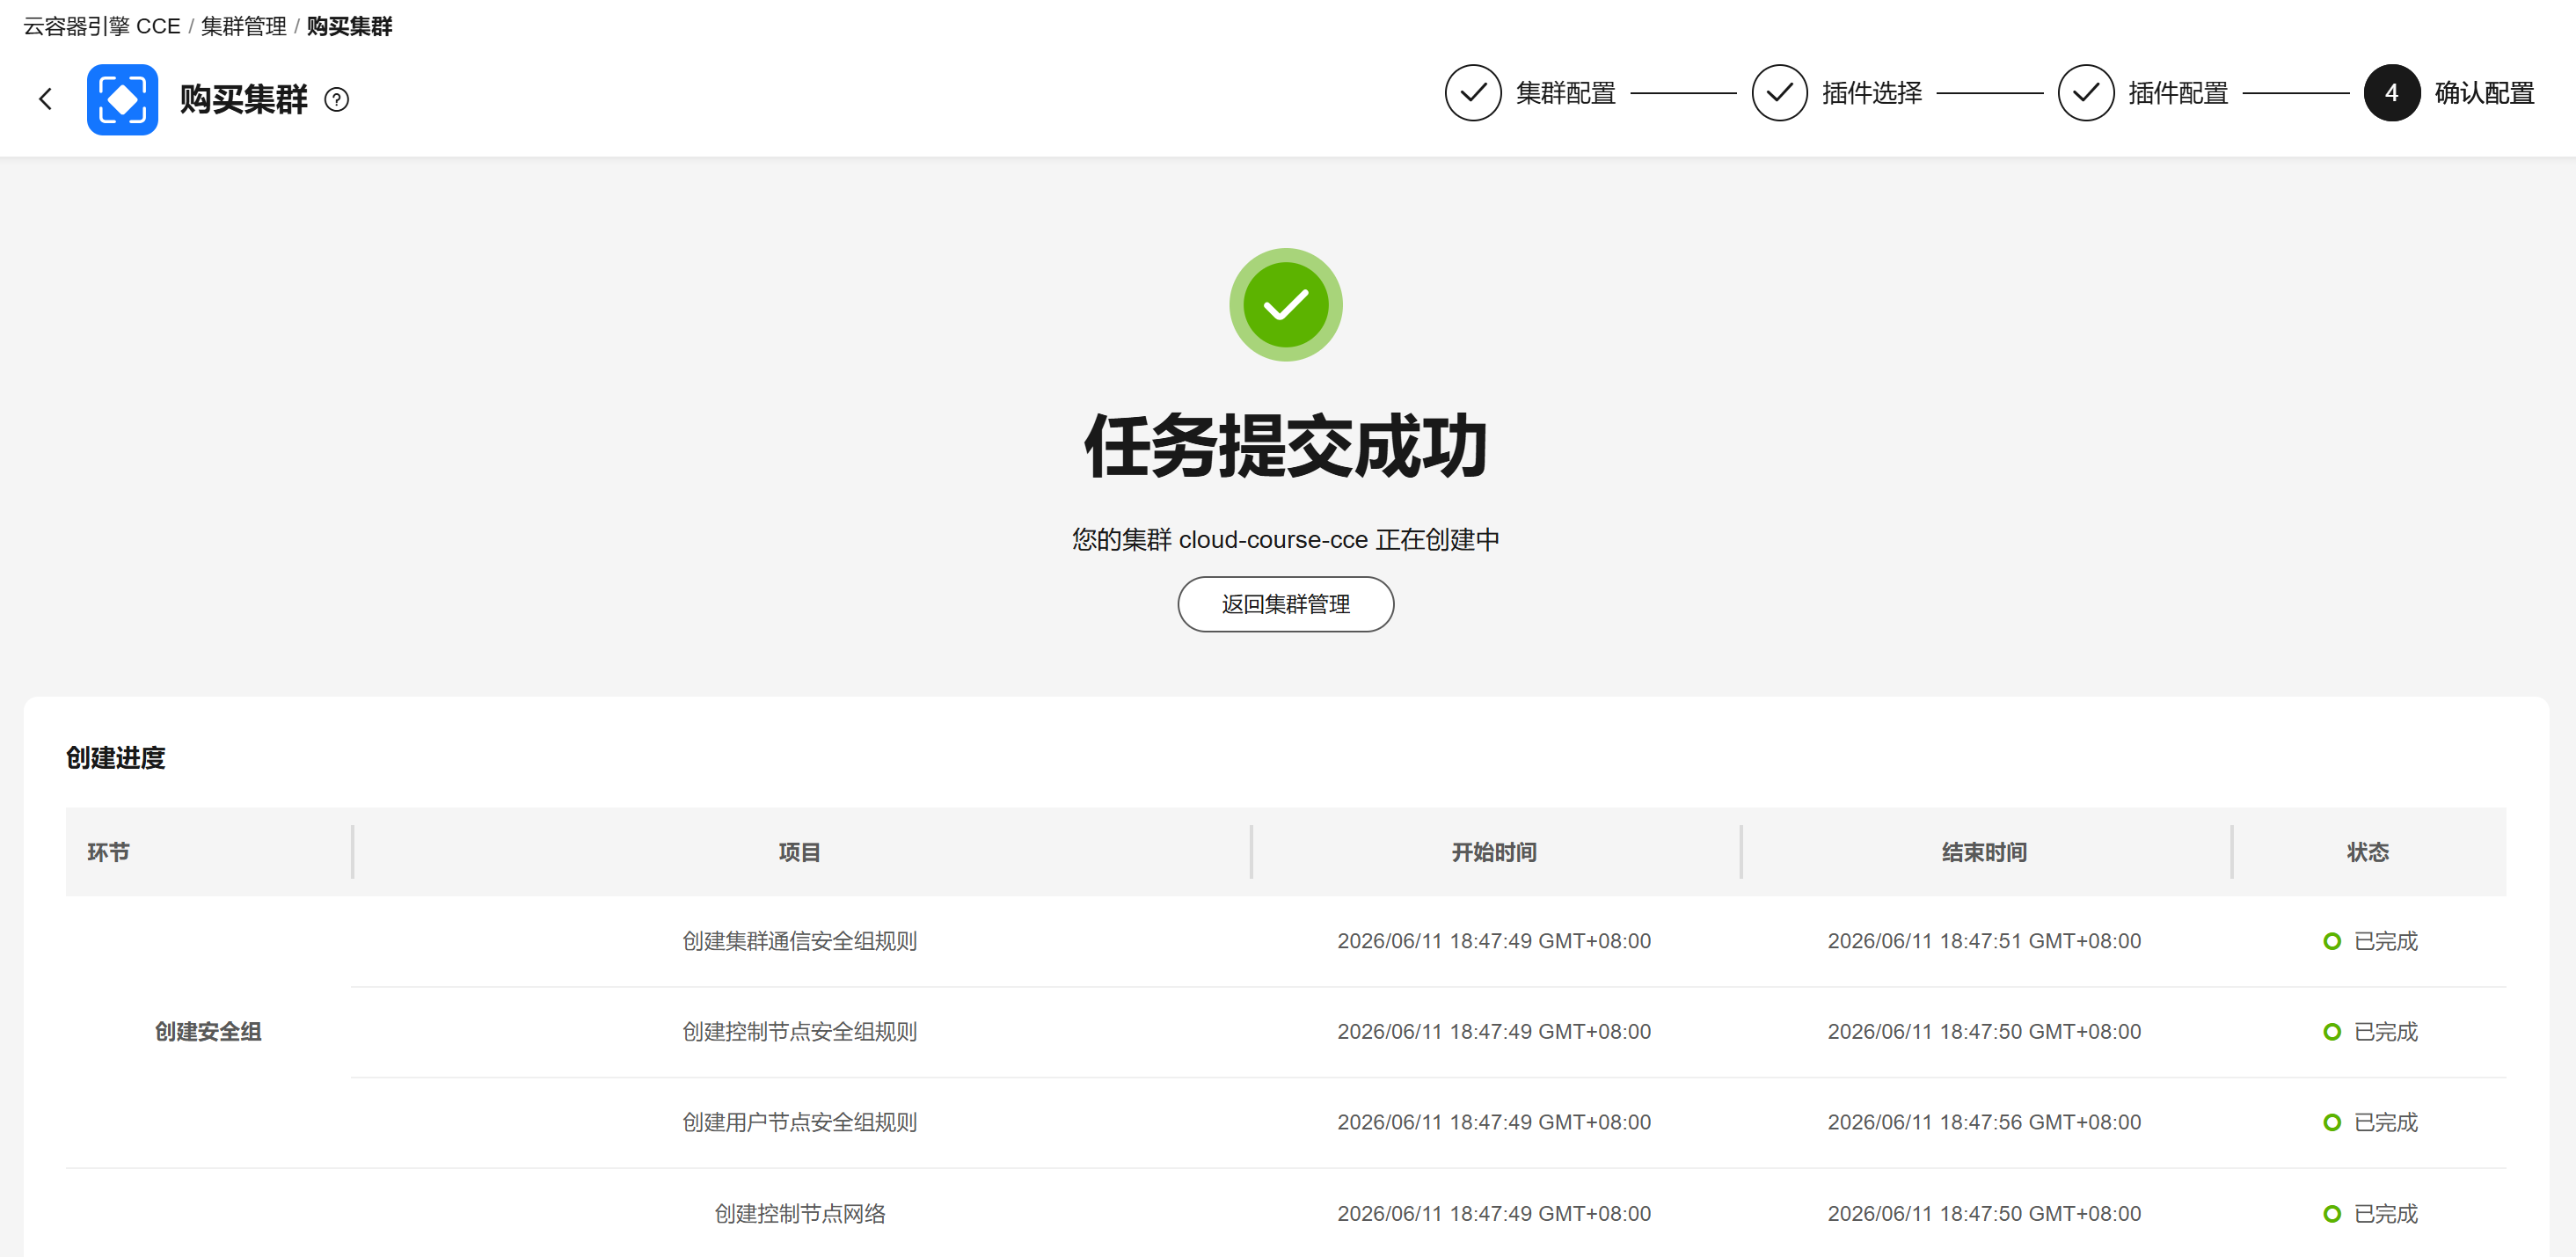
\includegraphics[width=0.92\textwidth]{assets/report_figures/t2/t2-13-cce-creating.png}
  \caption{CCE 集群进入创建中状态截图}
  \label{fig:t2-cce-creating}
\end{figure}

图 \ref{fig:t2-cce-creating} 显示 CCE 集群创建任务已经提交，并进入创建中状态。

\subsubsection{OBS数据存储配置}

OBS 对应 Spark 大数据分析中的数据存储场景，Spark 作业可以通过 \texttt{s3a://} 路径读取对象存储中的文件。本项目的 \texttt{spark/analysis.py} 支持把数据路径作为参数传入，因此既能读取仓库中的本地 \texttt{douban\_movies.csv}，也可以替换为 OBS 路径。当前截图材料中没有单独保存 OBS 控制台页面，因此这里不补放 OBS 截图，Spark 章节只围绕实际脚本和运行结果说明。

OBS 和 CCE 不是直接部署关系。CCE 负责运行 Spark Driver 和 Executor，OBS 只提供数据文件；作业运行时通过 S3A 协议读取数据，再完成 DataFrame 加载、清洗和 SQL 分析。

\subsubsection{ELB负载均衡配置}

ELB 用于对外暴露后端服务。Kubernetes 中的后端 Service 设置为 \texttt{LoadBalancer} 类型后，会绑定华为云 ELB，外部浏览器或 curl 才能访问 \texttt{/api/ping}。T3 验收时主要看公网访问是否返回正常 JSON。

\begin{figure}[H]
  \centering
  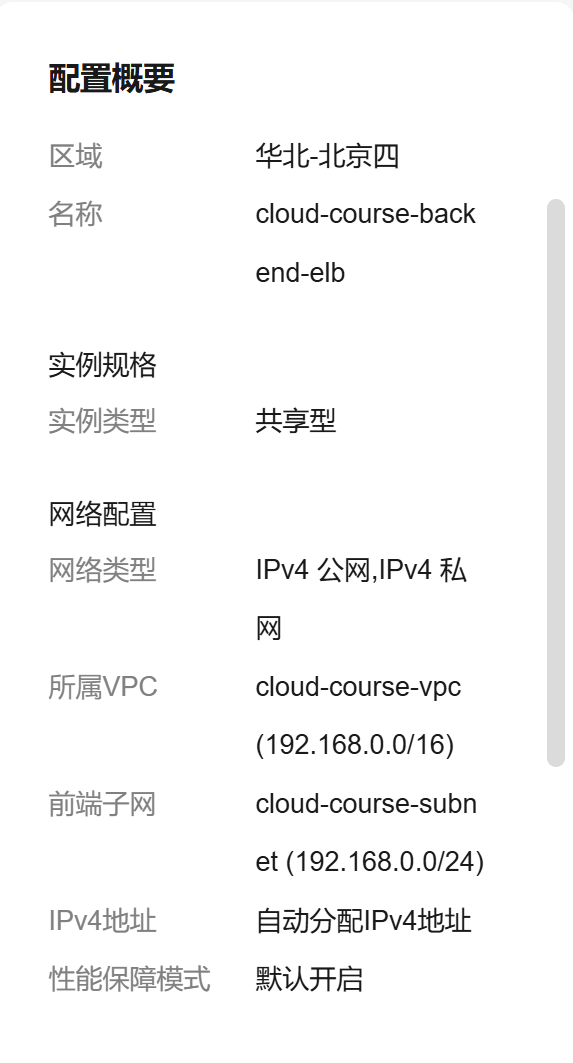
\includegraphics[width=0.65\textwidth]{assets/report_figures/env/env-elb-config.png}
  \caption{共享型公网 ELB 创建配置概要截图}
  \label{fig:env-elb-config}
\end{figure}

图 \ref{fig:env-elb-config} 展示了共享型公网 ELB 的创建配置。该负载均衡器用于后端 \texttt{backend-svc} 的公网访问入口，后续通过 Service 注解将 ELB 与 Kubernetes Service 绑定。

\begin{figure}[H]
  \centering
  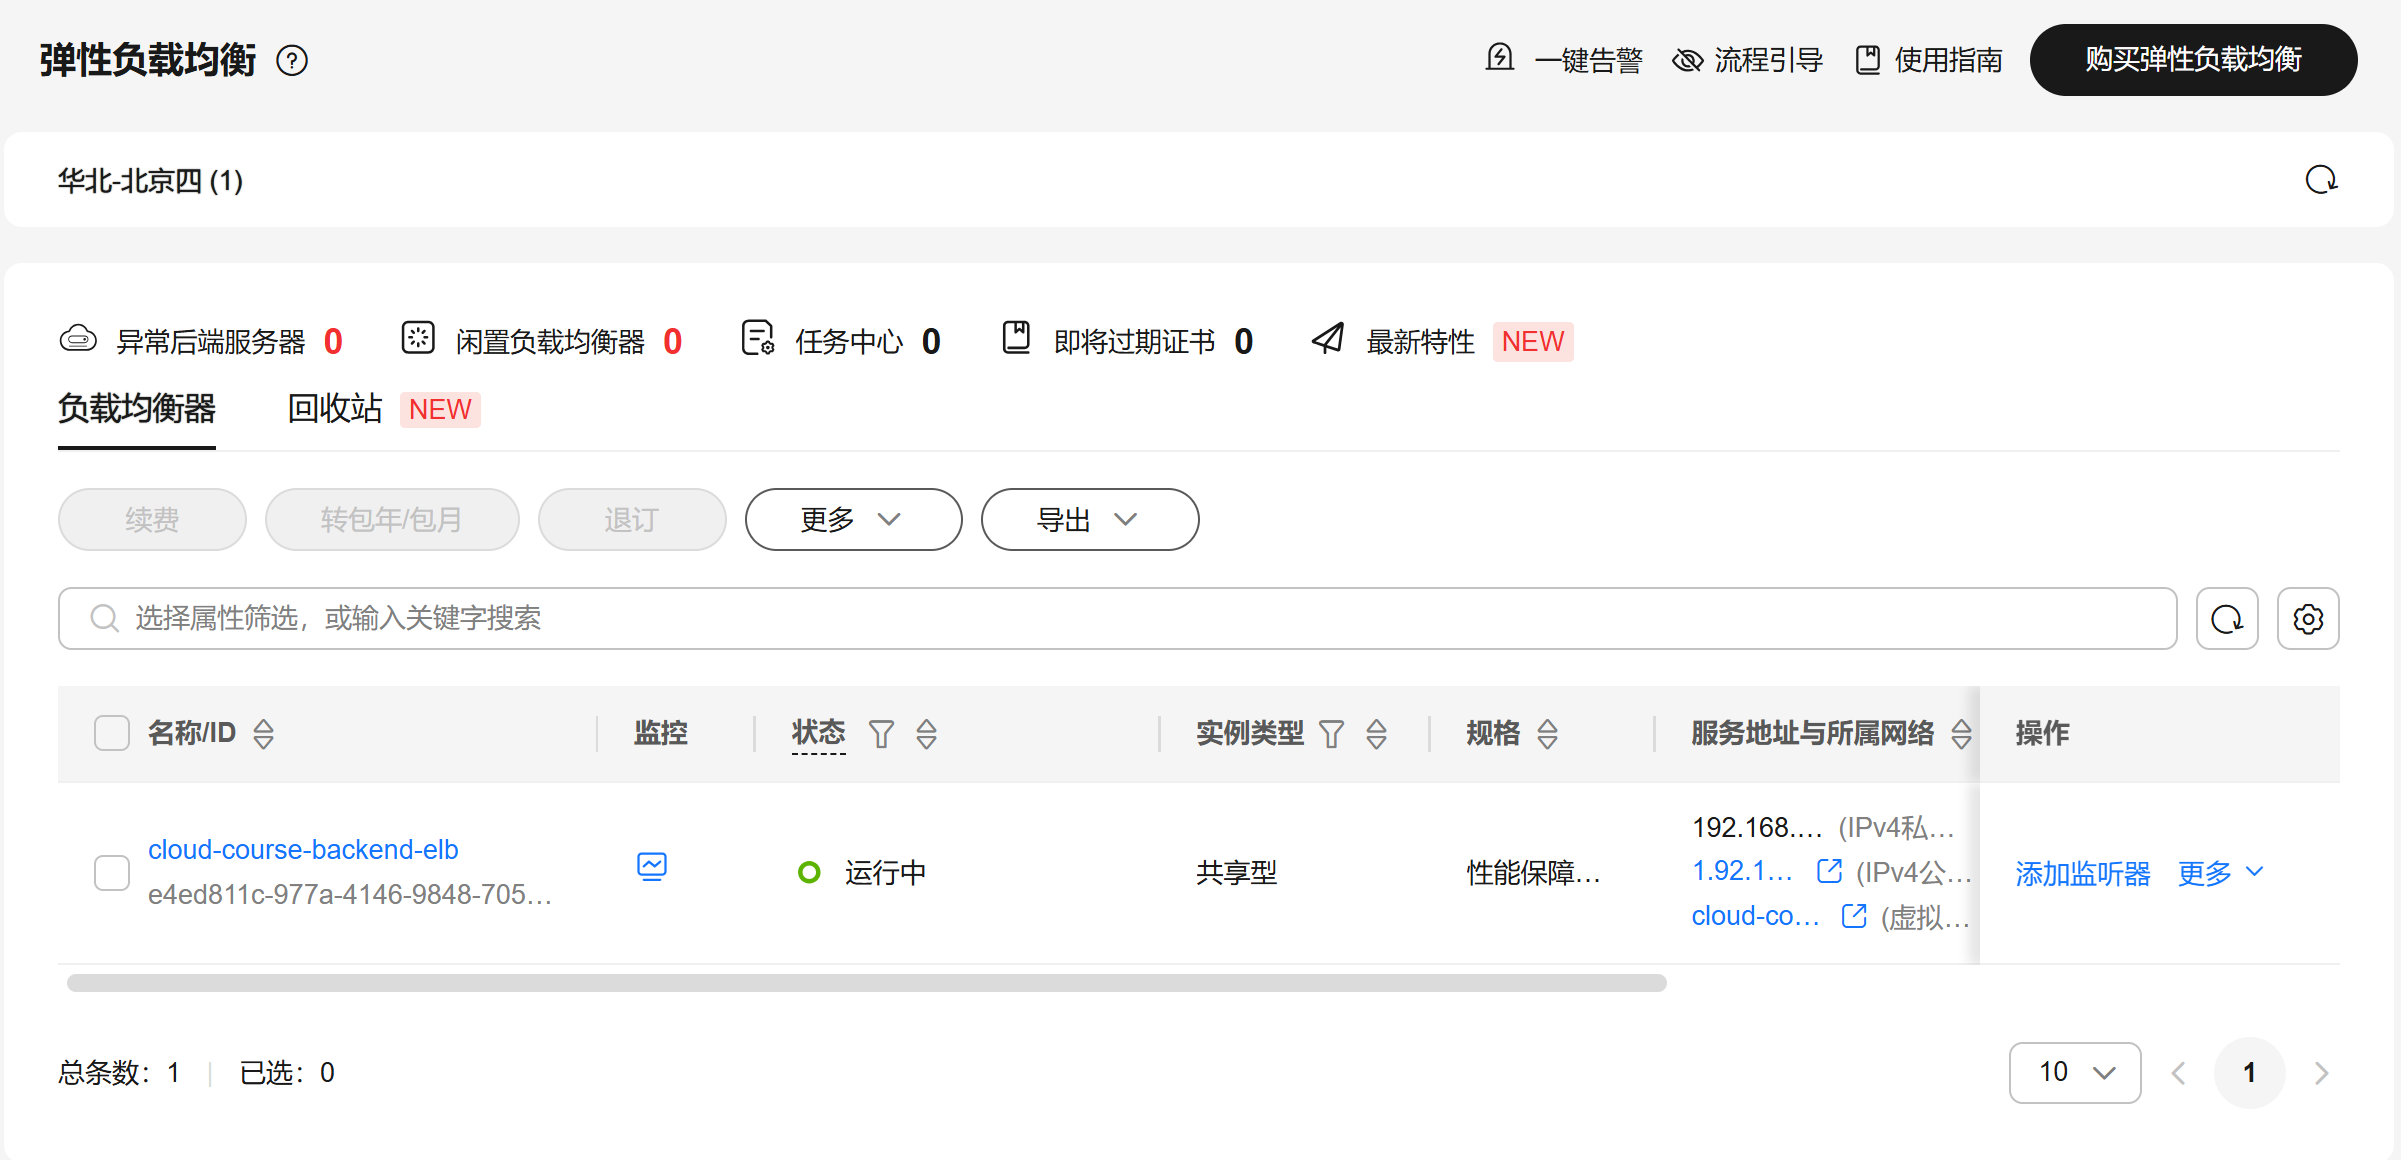
\includegraphics[width=0.92\textwidth]{assets/report_figures/env/env-elb-running.png}
  \caption{ELB 负载均衡器运行中状态截图}
  \label{fig:env-elb-running}
\end{figure}

图 \ref{fig:env-elb-running} 显示 ELB 资源已经创建并处于运行中状态。该状态说明公网负载均衡基础资源可用，为后续通过公网 IP 访问后端接口提供环境条件。

\subsection{Kubernetes集群信息}

T2 主要验收 Kubernetes 集群是否真正可用。集群创建完成后，我们分别在 CCE 控制台和 CloudShell 中检查了节点运行状态、kubectl 连接状态和客户端版本。相关环境参数见表 \ref{tab:k8s-cluster-info}。

\begin{table}[H]
  \centering
  \caption{Kubernetes 集群关键参数}
  \label{tab:k8s-cluster-info}
  \small
  \renewcommand{\arraystretch}{1.22}
  \begin{tabularx}{\textwidth}{>{\raggedright\arraybackslash}p{3.2cm} Y}
    \toprule
    项目 & 内容 \\
    \midrule
    区域 & 华北-北京四 \\
    集群名称 & \texttt{cloud-course-cce} \\
    集群类型 & CCE Standard \\
    计费模式 & 按需计费 \\
    Kubernetes 版本 & v1.34，节点输出中 VERSION 为 \texttt{v1.34.6-r0-34.0.23} \\
    Worker 节点数量 & 2 个 \\
    Worker 节点规格 & \texttt{c9.large.2}，2 vCPU / 4 GiB \\
    操作系统 & Ubuntu 22.04.5 LTS \\
    容器运行时 & containerd \\
    VPC / 子网 & \texttt{cloud-course-vpc} / \texttt{cloud-course-subnet} \\
    \bottomrule
  \end{tabularx}
\end{table}

\subsubsection{集群版本与节点规格}

集群版本和节点规格决定了后续 Kubernetes 资源是否能够稳定运行。本项目选择 v1.34 版本，显著高于任务书要求的 v1.27 下限；节点采用 2 vCPU / 4 GiB 规格，能够满足 Flask 后端、Redis、Nginx 前端以及基础 Spark Operator 验证的课程设计需求，同时控制云资源成本。

\begin{figure}[H]
  \centering
  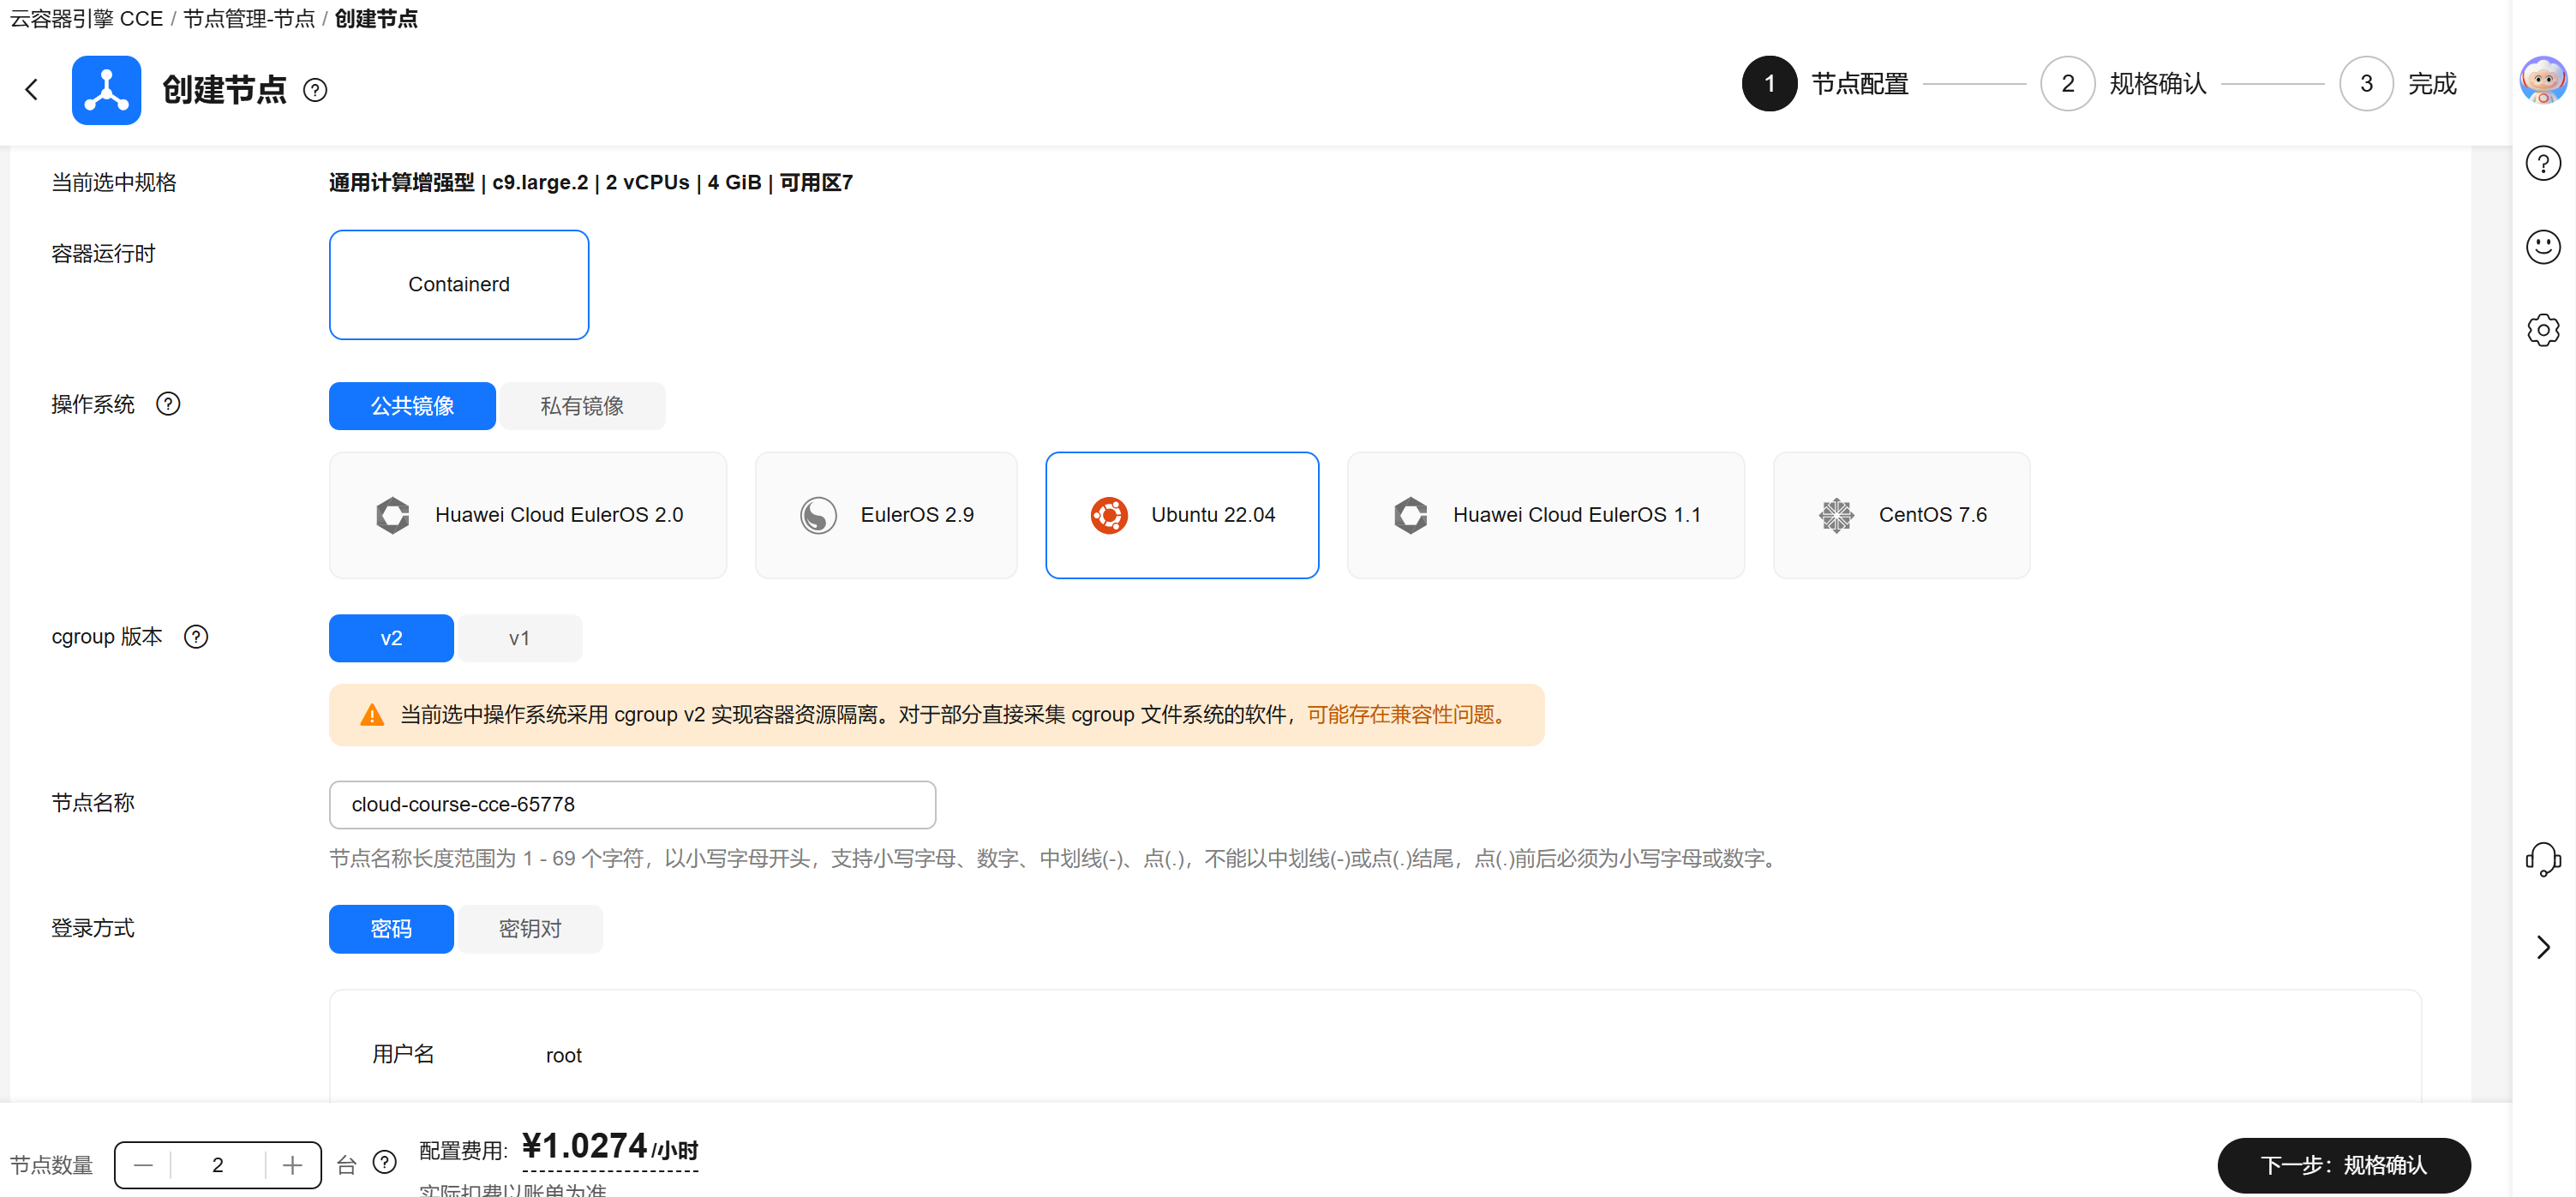
\includegraphics[width=0.92\textwidth]{assets/report_figures/t2/t2-14-worker-config-1.png}
  \caption{创建 Worker 节点时的基础规格配置截图}
  \label{fig:t2-worker-config-1}
\end{figure}

图 \ref{fig:t2-worker-config-1} 记录了 Worker 节点的基础规格配置，可以看出节点规格是按课程设计成本和运行需求手动选择的。

\begin{figure}[H]
  \centering
  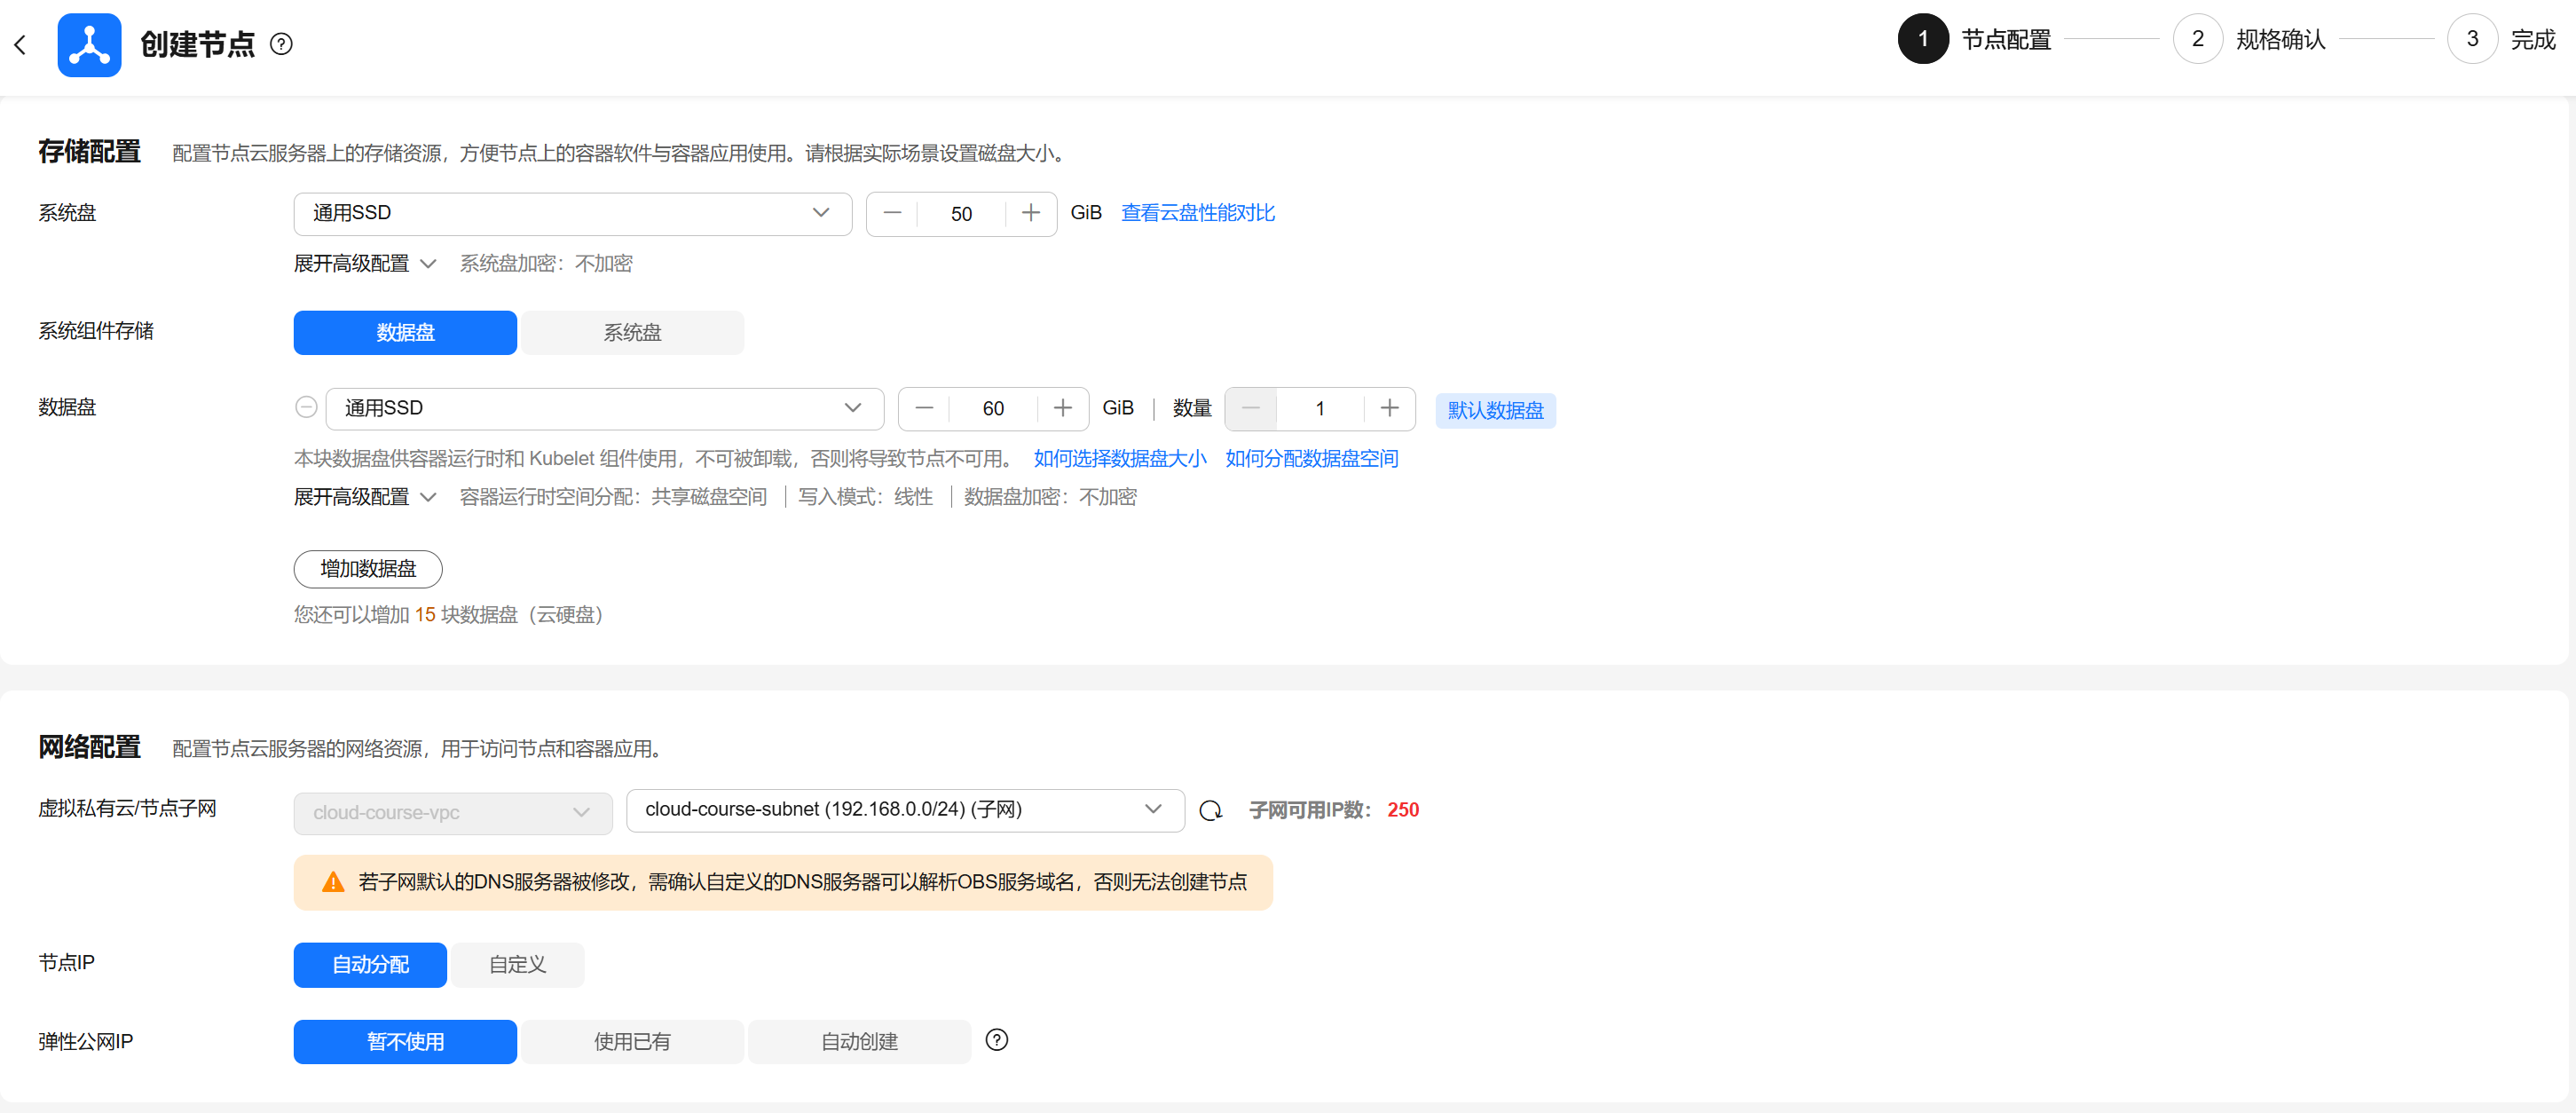
\includegraphics[width=0.92\textwidth]{assets/report_figures/t2/t2-15-worker-config-2.png}
  \caption{创建 Worker 节点时的存储与网络配置截图}
  \label{fig:t2-worker-config-2}
\end{figure}

图 \ref{fig:t2-worker-config-2} 展示了 Worker 节点创建过程中的存储与网络配置。该配置影响节点能否正常加入 VPC、能否创建容器运行环境，以及后续是否能够挂载存储卷。

\begin{figure}[H]
  \centering
  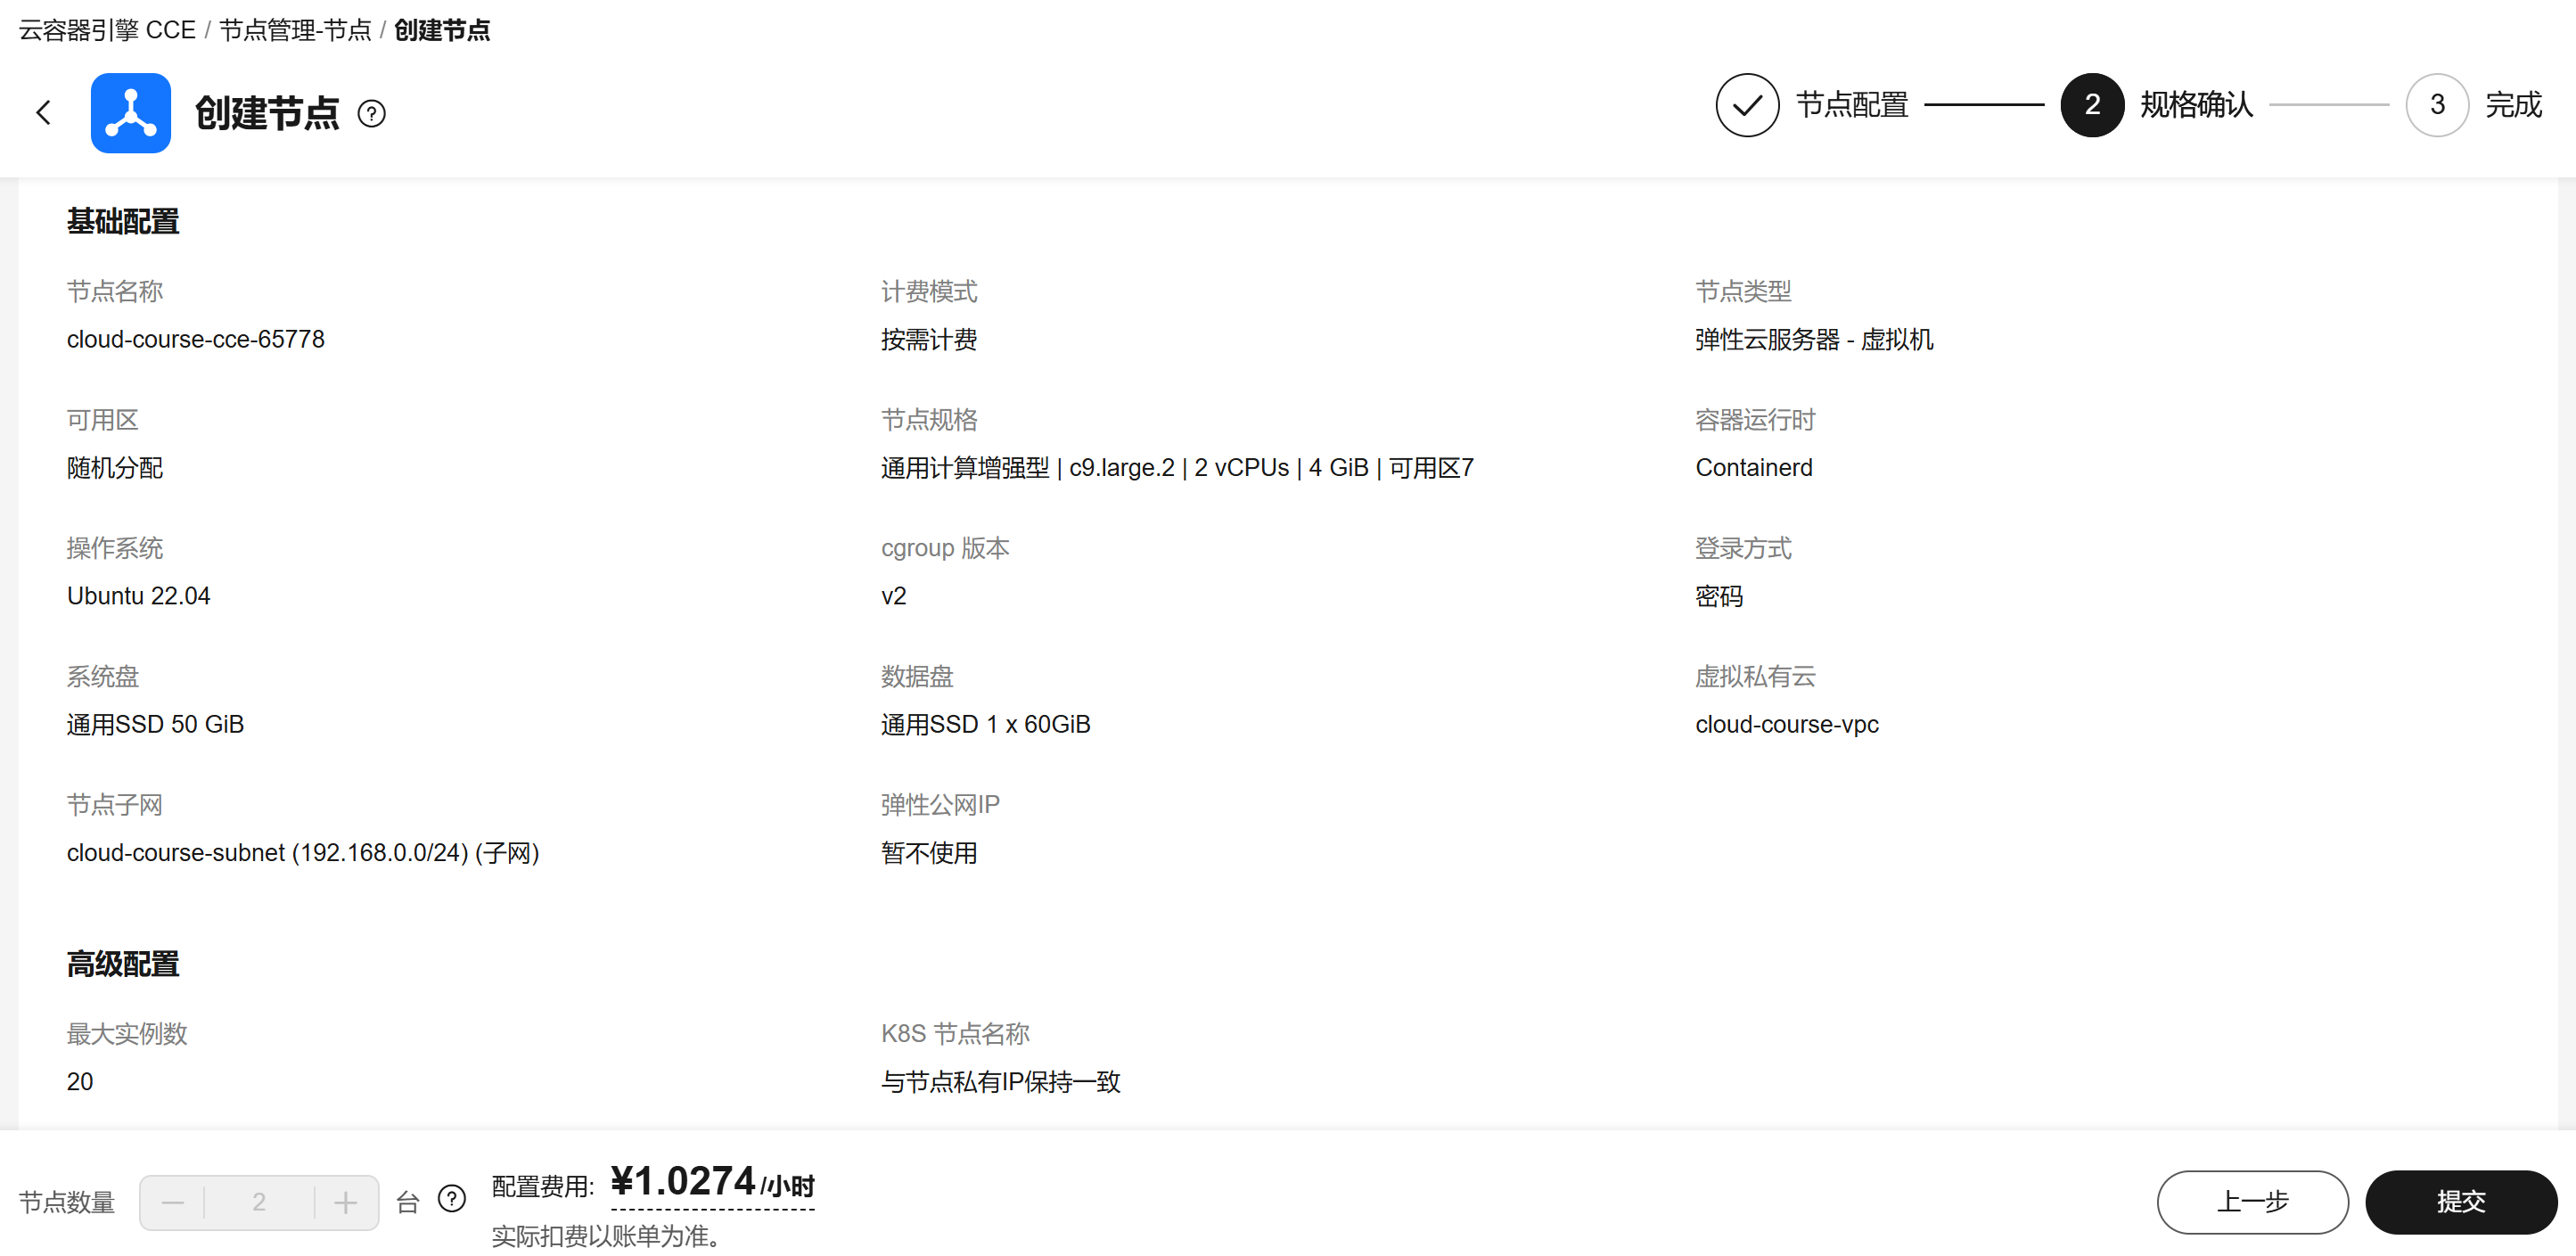
\includegraphics[width=0.92\textwidth]{assets/report_figures/t2/t2-16-worker-confirm.png}
  \caption{Worker 节点规格确认页面截图}
  \label{fig:t2-worker-confirm}
\end{figure}

图 \ref{fig:t2-worker-confirm} 是 Worker 节点规格确认页面，可以看到节点数量和规格。

\begin{figure}[H]
  \centering
  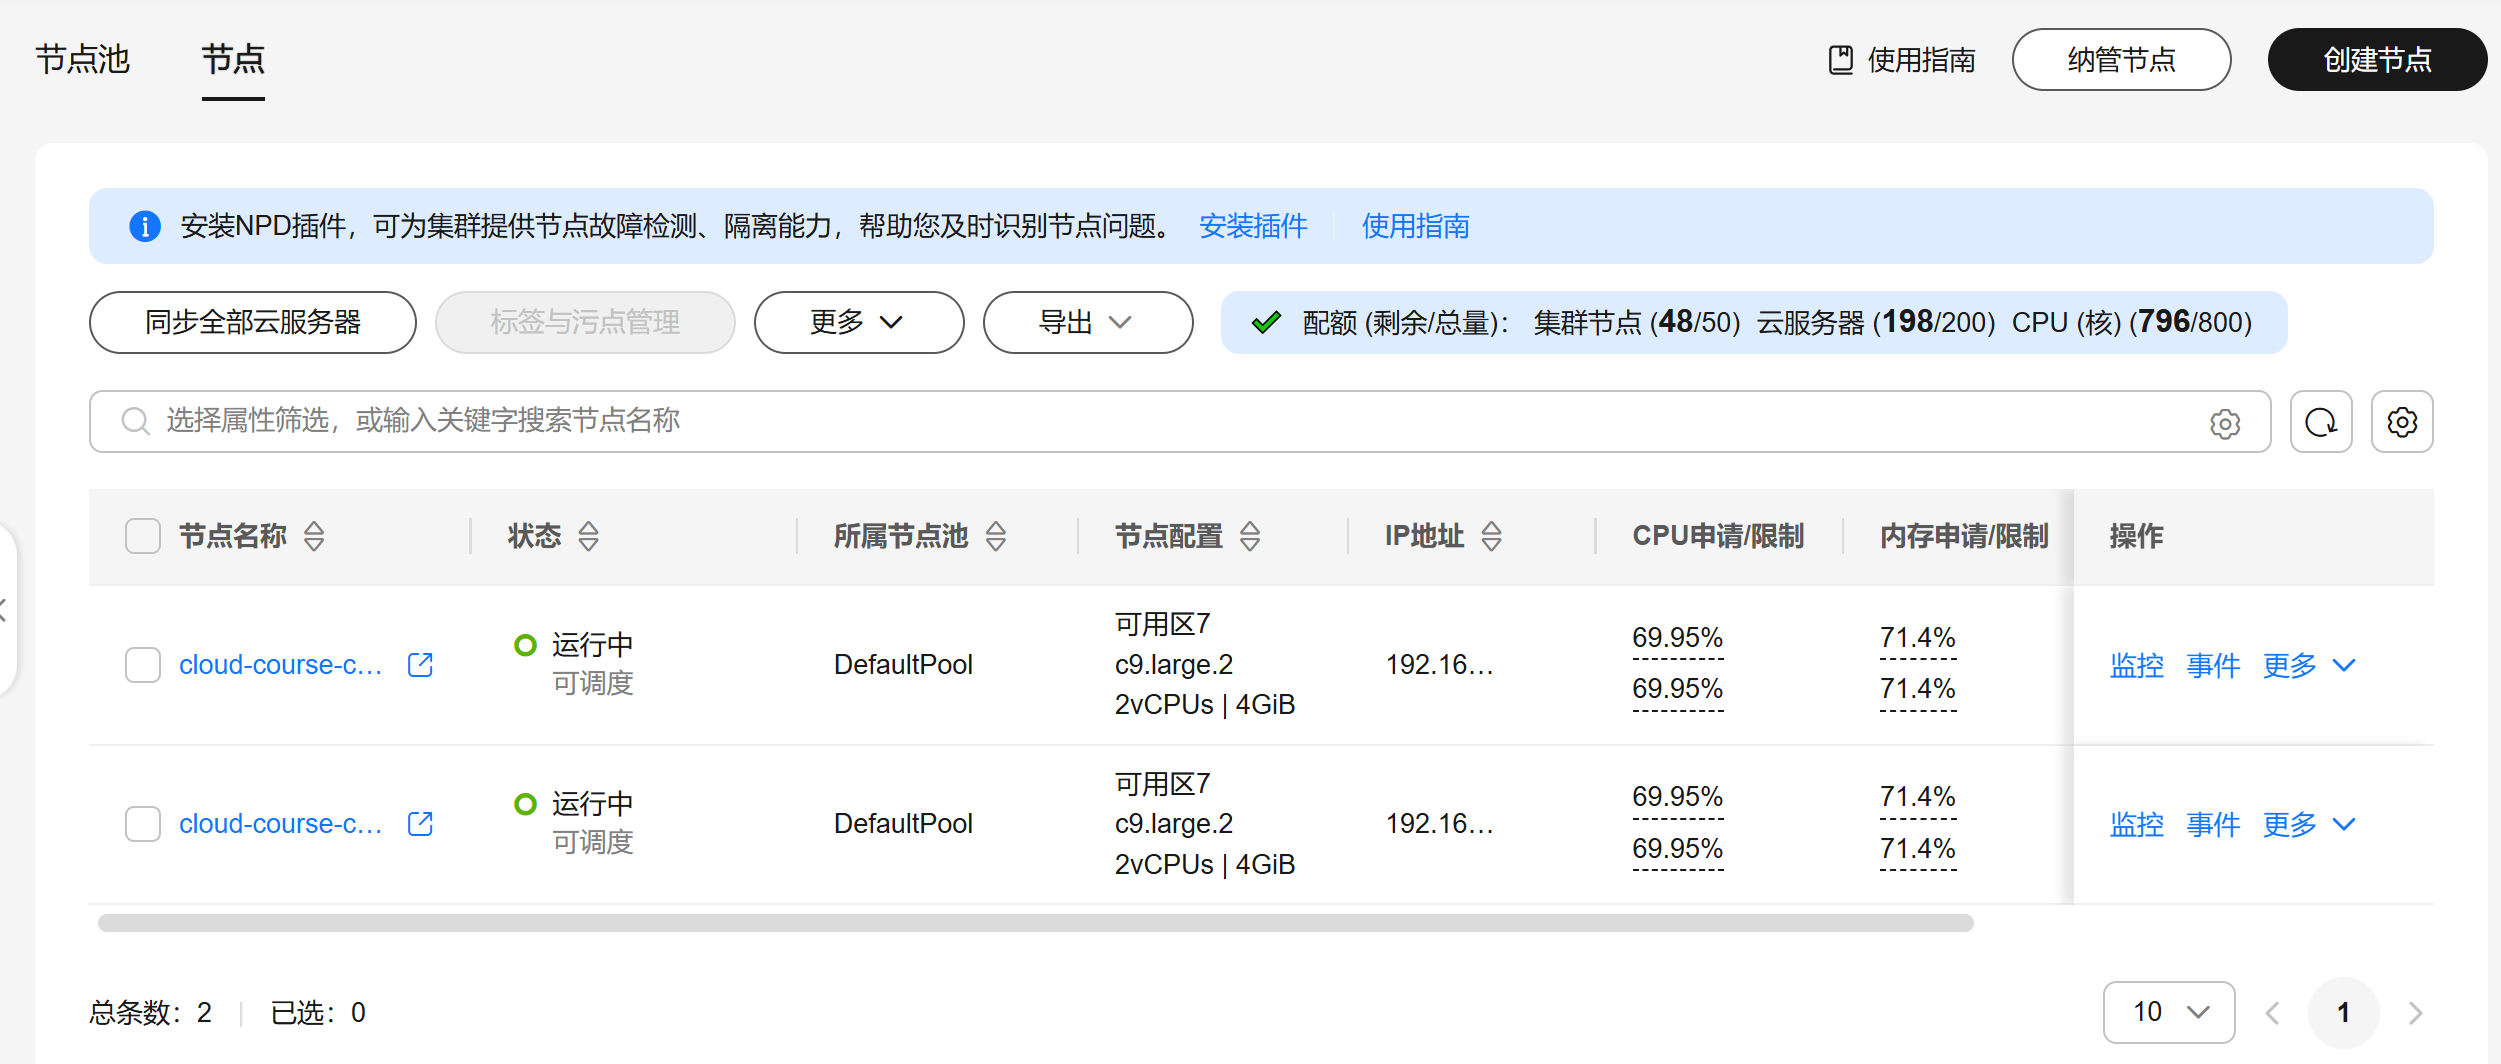
\includegraphics[width=0.92\textwidth]{assets/report_figures/t2/t2-17-worker-running.png}
  \caption{CCE 控制台显示两个 Worker 节点运行中截图}
  \label{fig:t2-worker-running}
\end{figure}

图 \ref{fig:t2-worker-running} 显示 CCE 控制台中两个 Worker 节点处于运行中状态，说明节点已经创建成功。

\subsubsection{kubectl连接与节点状态}

创建集群后，需要配置 kubectl 才能对 Kubernetes 集群执行资源管理操作。本项目使用华为云 CloudShell 配置 kubectl，并通过 \texttt{kubectl get nodes -o wide} 验证两个 Worker 节点均为 Ready。该命令输出同时包含节点名称、状态、角色、版本、内网 IP、操作系统和容器运行时等信息，是任务书 T2 的核心验收截图。

\begin{figure}[H]
  \centering
  {\setlength{\fboxsep}{0pt}\setlength{\fboxrule}{1.2pt}\fcolorbox{red}{white}{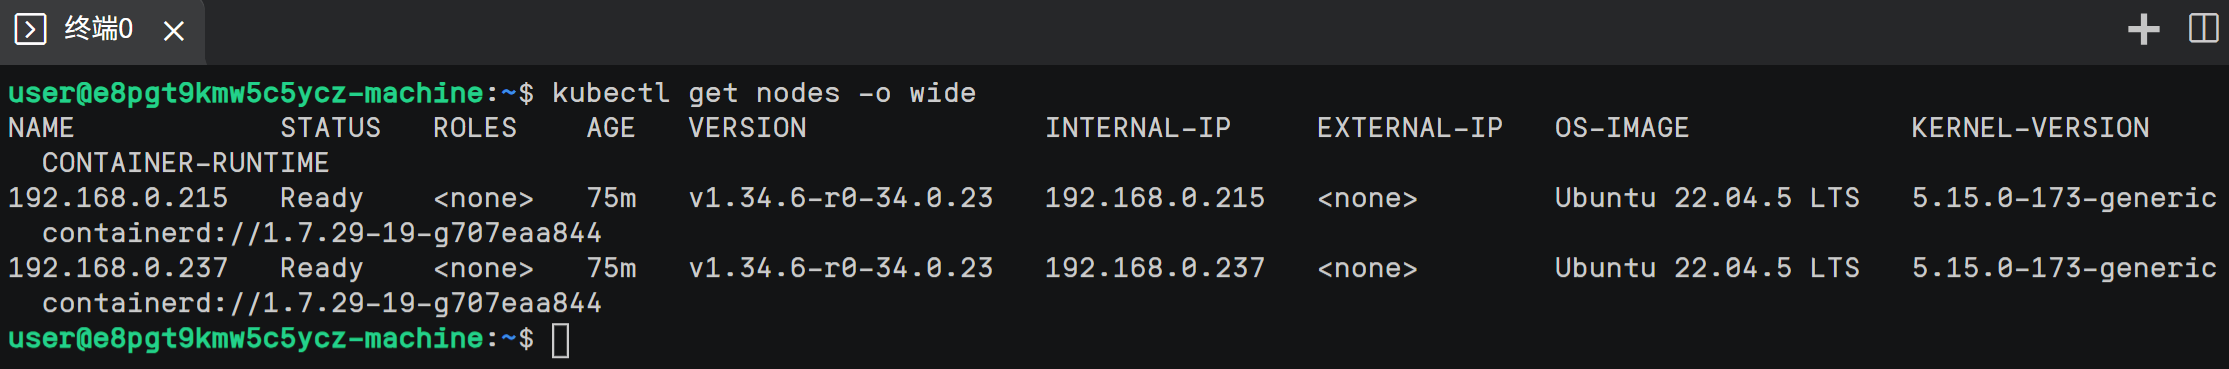
\includegraphics[width=0.88\textwidth]{assets/report_figures/t2/t2-18-nodes-ready.png}}}
  \caption{核心验收：kubectl 查看两个 Worker 节点 Ready 状态截图}
  \label{fig:t2-nodes-ready}
\end{figure}

图 \ref{fig:t2-nodes-ready} 使用红框突出显示核心验收截图。截图中可以看到两个 Worker 节点的 \texttt{STATUS} 均为 \texttt{Ready}，\texttt{VERSION} 列为 \texttt{v1.34.6-r0-34.0.23}，节点内网 IP 分别为 \texttt{192.168.0.215} 和 \texttt{192.168.0.237}。这说明集群节点已经成功加入 Kubernetes，并且版本满足任务书要求。需要说明的是，CCE Worker 节点在 \verb|kubectl get nodes -o wide| 输出中 \texttt{ROLES} 列可能显示为 \verb|<none>|，这是华为云 CCE 托管集群中的常见现象，并不表示节点未就绪；T2 验收以 \texttt{STATUS=Ready} 及 \texttt{VERSION} 列是否满足版本要求为准。

\begin{figure}[H]
  \centering
  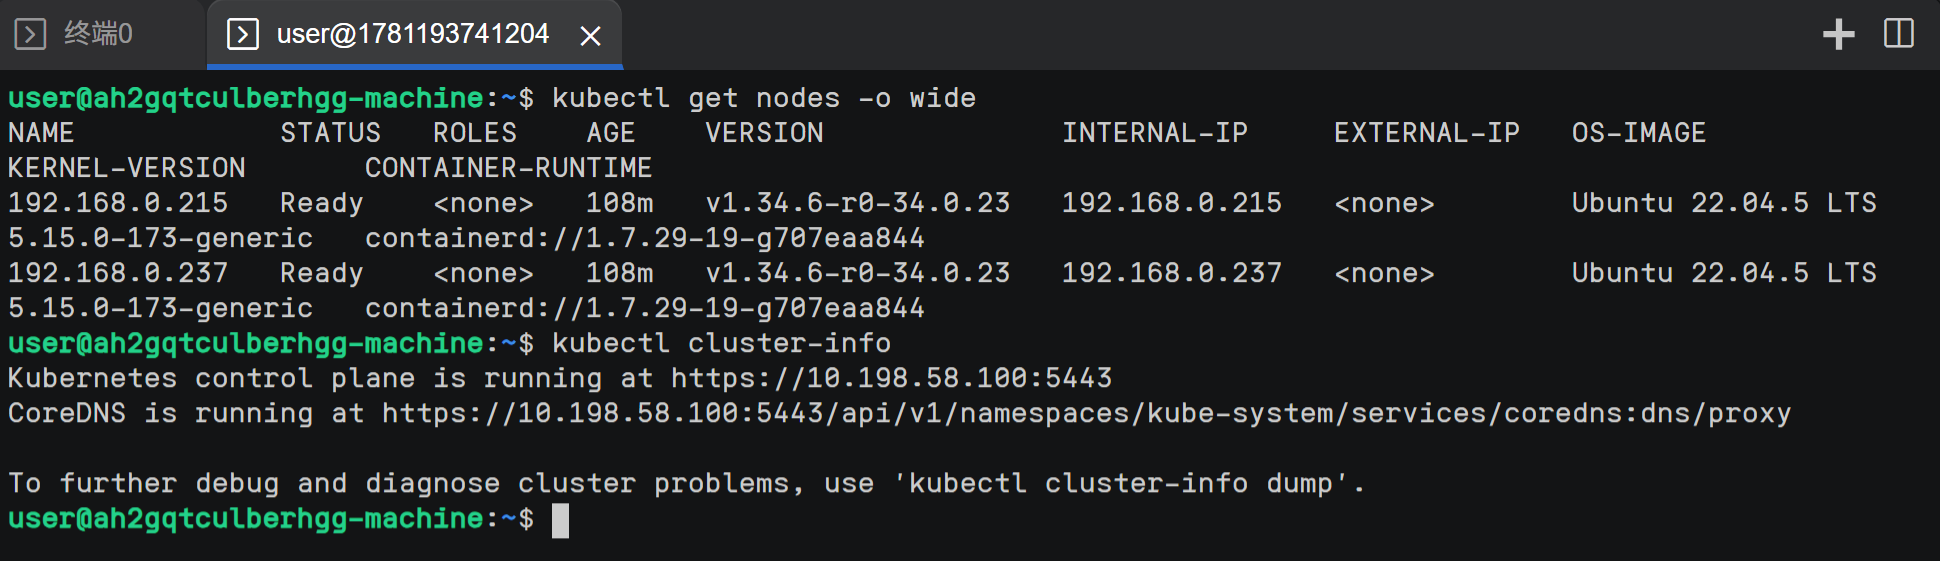
\includegraphics[width=0.92\textwidth]{assets/report_figures/t2/t2-19-cluster-info.png}
  \caption{kubectl cluster-info 连接集群成功截图}
  \label{fig:t2-cluster-info}
\end{figure}

图 \ref{fig:t2-cluster-info} 给出了 \texttt{kubectl cluster-info} 的输出。能看到控制平面地址后，后续才可以继续通过 \texttt{kubectl apply} 部署 YAML 资源。

\begin{figure}[H]
  \centering
  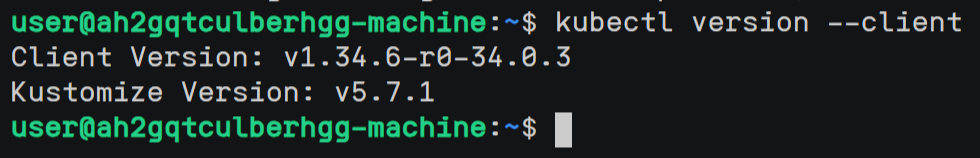
\includegraphics[width=0.92\textwidth]{assets/report_figures/t2/t2-20-kubectl-version.png}
  \caption{kubectl 客户端版本信息截图}
  \label{fig:t2-kubectl-version}
\end{figure}

图 \ref{fig:t2-kubectl-version} 展示了 CloudShell 中 kubectl 客户端版本信息。该截图说明实验环境中 kubectl 工具可用，且后续对 Pod、Service、PVC 和 HPA 的管理均可通过命令行完成。

\subsubsection{命名空间与资源规划}

本项目基础任务主要使用 Kubernetes 的 \texttt{default} 命名空间，便于课程设计验收时统一查看 Pod、Deployment、Service、ConfigMap、Secret、PVC 和 HPA 等资源。后端 Deployment 命名为 \texttt{backend}，Redis Deployment 命名为 \texttt{redis}，前端 Deployment 命名为 \texttt{frontend}；后端 Service 命名为 \texttt{backend-svc}，Redis Service 命名为 \texttt{redis-svc}，前端 Service 命名为 \texttt{frontend-svc}。配置资源方面，后端使用 \texttt{backend-config} 注入 Redis 地址和端口，使用 \texttt{redis-secret} 保存 Redis 密码字段；持久化存储方面，Redis 使用 \texttt{redis-data-pvc} 申请云硬盘存储。

资源命名尽量和任务书中的组件名称保持一致，便于截图核对。敏感配置放入 Secret，普通配置放入 ConfigMap；对外访问只开放后端 LoadBalancer Service，Redis 保持 ClusterIP 内部访问。Spark Operator 和监控系统需要单独命名空间时，在对应实验步骤中再创建。
